\documentclass{article}
\usepackage{caption}
\usepackage{algorithm2e}
\usepackage{authblk}
\usepackage{graphicx}
\usepackage{listings}
\usepackage{array}
\usepackage{courier}
\usepackage{csquotes}
\usepackage[USenglish]{babel}
\usepackage{nameref}
\usepackage{makecell}

\usepackage[backend=bibtex,sorting=none]{biblatex}
\addbibresource{manuscript}
\graphicspath{{assets/images/}}
\emergencystretch=1em
\DeclareUnicodeCharacter{2212}{-}

\def\ttt{\texttt}

\begin{document}

\hyphenation{organo-metallics Proto-SMILES}
\newcolumntype{L}{>{\arraybackslash}m{3cm}}
\lstset{basicstyle=\ttfamily,breaklines=true}


\title{Balsa: A Compact Line Notation Based on SMILES}
\author{Richard L. Apodaca\thanks{rapodaca@metamolecular.com}}

\maketitle

\section*{Introduction}

Simplified Molecular Input Line Entry System (SMILES) was first described by Weininger in 1988~\cite{weininger:1988}. As a line notation~\cite{wiswesser:1968}, SMILES represents molecules as single line character sequences, or strings. SMILES has since been widely adopted. Read and write functionalities are routinely supported by popular cheminformatics toolkits, including: Open Babel~\cite{oBoyle:2011}; RDKit~\cite{rdkit}; Chemistry Development Kit~\cite{steinbeck:2003}; JChem Base~\cite{jchemBase}; the Daylight Toolkit~\cite{daylightToolkit}; and OEChem TK~\cite{oetk}. SMILES encodings can be found in many public-facing databases, including: PubChem~\cite{kim:2016}; ChEBI~\cite{degtyarenko:2007}; ZINC~\cite{irwin:2005}; ChEMBL~\cite{gaulton:2012}; and Wikipedia~\cite{wikipediaCAS}. Raw SMILES strings have been used extensively in machine learning applications~\cite{sousa:2021}. Algorithmic selection of a single SMILES encoding has been used for unique molecular identification~\cite{weininger:1989,oBoyle:2012}. SMILES has also been extended to carry various forms of metadata, as exemplified by Jmol SMILES~\cite{hanson:2016}, CurleySMILES~\cite{drefahl:2011}, BigSMILES~\cite{lin:2019}, and CXSMILES~\cite{cxsmiles}.

Despite the central role that SMILES plays in cheminformatics, public descriptions of the language remain imprecise at best. A 1987 report to the US Environmental Protection Agency by Weininger described a language similar to SMILES, but with important differences~\cite{anderson:1987}. Weininger's 1988 paper offered an overview of the language, but omitted or only partially addressed points crucial to correctly implementing SMILES, including: (1) stereochemical configuration; (2) double bond conformation; (3) the encoding and decoding of \enquote{aromatic} features; (4) the computation of implicit hydrogen count, especially in the context of aromatic features; (5) formal syntax; (6) constraints on quantities such as mass number and charge; and (7) enumeration of error states.

Since 1988, two authoritative sources have attempted to clarify or revise Weininger's 1988 description of SMILES. A 2003 book chapter by Weininger addressed some of the limitations of the paper~\cite{weininger:2003}. The Daylight Theory Manual, a website maintained by SMILES's corporate sponsor, Daylight Chemical Information Systems, Inc. (\enquote{Daylight}), recapitulates previously-published material~\cite{daylightTheory}. The lack of other authoritative sources describing SMILES is consistent with Weininger's reported disinterest in traditional scientific publication~\cite{gasteiger:2018}.

In 2007 a documentation effort that would become known as OpenSMILES began~\cite{openSMILES}. OpenSMILES was conceived as \enquote{a non-proprietary specification for the SMILES language.} Many of the points left open by previous SMILES documentation efforts were addressed. Noteworthy contributions included: the first formal grammar, later adapted to a standard parser toolchain~\cite{denjoed:2010}; many refinements around stereochemistry; and the introduction of \enquote{standard form.} Absent were detailed procedures for assigning and interpreting aromatic features, and a detailed procedure for computing implicit hydrogen count. OpenSMILES also left several points of syntactic and semantic ambiguity unsettled, while introducing extensions of its own.

In 2019 IUPAC announced the SMILES+ initiative~\cite{smilesPlusSpecification}. Noting the limitations of existing SMILES documentation, the SMILES+ effort seeks to \enquote{establish a formalized recommended up-to-date specification of the SMILES format.} SMILES+ took as its starting point the documentation produced by the OpenSMILES project. Efforts to extend this starting point are in progress online through a public repository, but no formal recommendation has to date resulted~\cite{smilesPlusGitHub}.

The lack of a comprehensive SMILES specification has caused several immediate problems. Maintainers of SMILES implementations lack a blueprint for working toward a common set of features and behaviors. At the same time, authors of new SMILES implementations must address ambiguities on an ad hoc basis. The diversity of implementations combined with language underspecification leaves standards bodies with a limited pool of source material upon which to draw. Widespread divergence around the edges of the SMILES language hampers the development of compliance suites, which only amplifies the problems faced by software teams trying to build compliant software. Finally, extensions to SMILES only make sense in the context of a rigorously defined base language.

More broadly, this situation undermines ongoing data integrity efforts underway in other scientific disciplines. For example, the FAIR Guiding Principles identify four qualities essential for extracting maximum utility from published scholarly data: Findability; Accessibility; Interoperability; and Reusability~\cite{wilkinson:2016}. The lack of a well-developed standard means that chemical data sets based on SMILES will suffer in all four areas.

The very notion of a SMILES standard may not be realistic at this point. Today a dozen or more slightly different implementations are in use. None of them can be considered a reference standard. Some have introduced extensions not recognized by the others, contributing to language drift while compounding the already formidable difficulties faced by implementors. Others claim SMILES compatibility while ignoring certain aspects of the documentation that does exist. The Daylight implementation, like some of the others, is distributed under a commercial license that restricts use~\cite{daylightToolkit}, and a publicly-accessible web service operated for many years has been decommissioned~\cite{depictArchive}. Although SMILES may underpin a lot of modern chemical information exchange, the foundations of this system are weathered and showing signs of stress.

This paper attempts to solve these problems with Balsa, a fully-specified language designed as a subset of SMILES. The following sections present Balsa from three perspectives: as a compact system for molecular representation; as a text-based language; and as a specification for software capable of the lossless conveyance of chemical structure information across organizational and temporal boundaries.

\section*{Goals}

Balsa's main goal is to solve the \textit{molecular serialization} problem. Serialization refers to the process of translating a data structure into a format that can be transmitted over a communication channel for later reconstruction. This allows general-purpose devices and networks to convey complex pieces of domain-specific information. Receiver and recipient may be separated by time, space, or both. Molecular serialization extends the concept of serialization to molecular structure. Examples of molecular serialization formats other than SMILES include Chemical Markup Language (CML)~\cite{murray-rust:2011}, CDXML~\cite{cdxml}, and CTfile (\enquote{molfile})~\cite{ctfileFormats}.

A secondary goal is brevity. Molecules should be expressable using only a few characters for each atom and either zero or one character for each bond. Brevity benefits humans who manually encode chemical structures within interactive line-driven interfaces such as those found in terminal sessions and notebooks. Brevity also benefits computers, for which compact molecular representation can improve the performance when storage, bandwidth, or processor cycles are limiting factors. Figure~\ref{fig:representative-examples} presents some simple chemical structures together with their Balsa serializations.

Molecular serialization schemes need to balance generality against complexity. As the diversity of the molecules that can be encoded increases, so do the rules needed to encode them and the software needed to interpret the rules. For this reason, Balsa's capabilities are directed at that region of chemical space populated by small organic molecules. Although Balsa can be used to represent a variety of other kinds of molecules, doing so in general risks data loss or corruption.

\begin{figure}
\centering
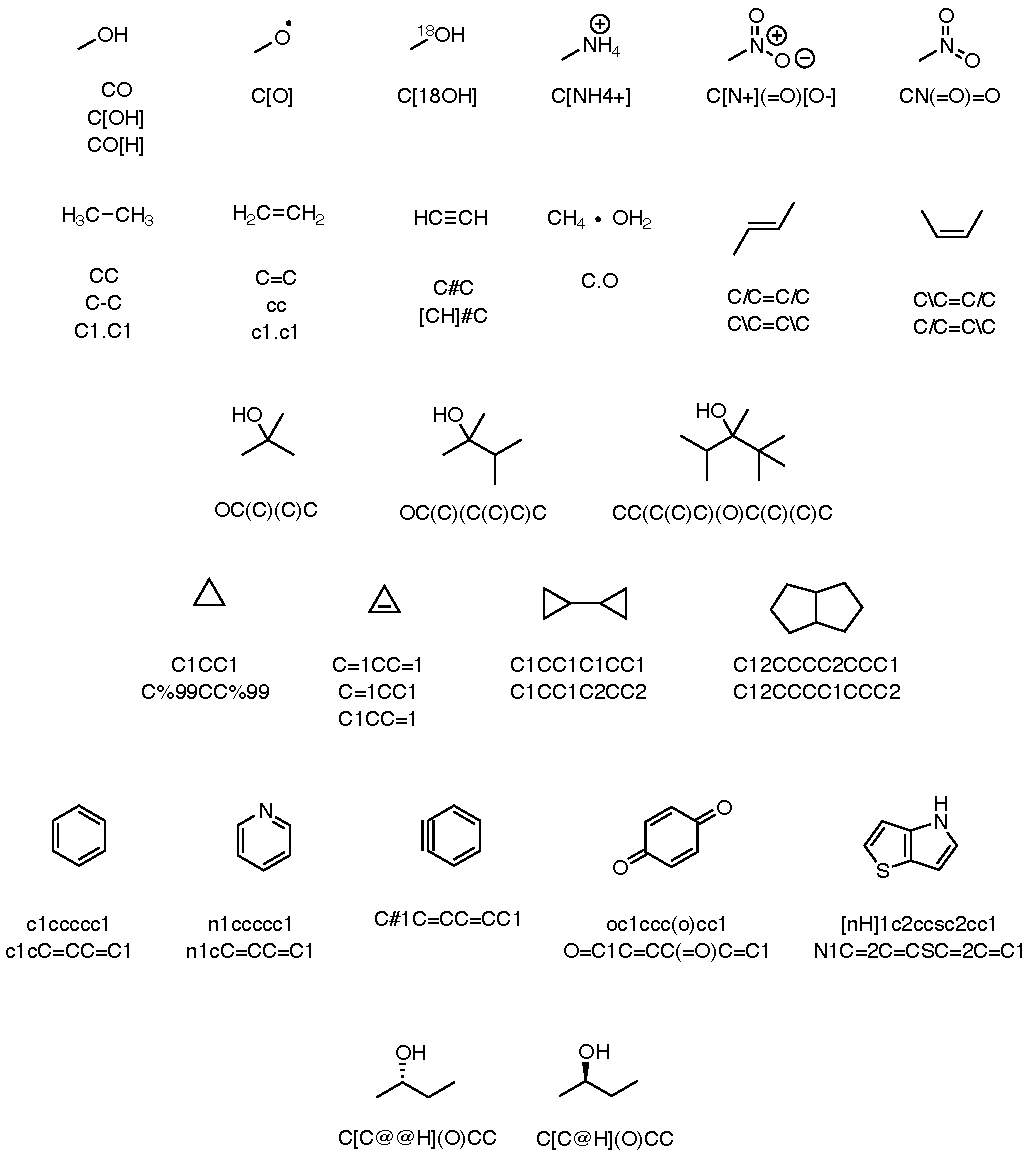
\includegraphics[width=\columnwidth]{representative-examples.pdf}
\caption{Representative Balsa examples.}
\label{fig:representative-examples}
\end{figure}

\section*{Molecular Representation}
\label{molecular-representation}

Balsa's rules can be divided into two broad categories: \textit{syntax} and \textit{semantics}. Syntax defines the set of valid strings for a language, whereas semantics determine the meaning these strings. Balsa semantic are complex due to the brevity of its syntax and the inherently complex nature of molecular representation.

Underpinning molecular serialization are conventions and abstractions for molecular representation. These are divided into three broad categories:

\begin{itemize}
\item \textit{Constitution}, the atoms present in a molecule and their bonding relationships. Balsa's extends the valence bond model with a limited form of delocalized bonding.
\item \textit{Conformation}, a kind of stereoisomerism resulting from restricted rotation about a bond. Balsa supports restricted rotation about double bonds capable of producing alkene isomerism.
\item \textit{Configuration}, a kind of stereoisomerism resulting from the arrangement of neighboring atoms in three-dimensional space. Balsa supports configurations for atoms having tetrahedral symmetry attached to four neighboring atoms.
\end{itemize}

\subsection*{Molecular Tree}
\label{molecular-tree}

Balsa represents molecular structure as a \textit{molecular tree} (Figure~\ref{fig:molecular-graph-vs-tree}). A tree is a data structure comprised of a set of nodes and pairwise relationships between them called edges. Any two nodes in a tree are connected through exactly one path of alternating nodes and edges. As such, a tree contains no cycles and exactly one connected component. A molecular tree is a specialized tree onto which chemically-relevant metadata have been overlaid. A Balsa molecule is a molecular tree having zero or more nodes and zero or more edges. The empty molecule, devoid of atoms and bonds, is therefore allowed. There is no upper bound on the number of nodes or edges, although limitations in hardware and software may restrict maximum molecular size.

A related but more common concept is the \textit{molecular graph}~\cite{balaban:1985}. Unlike molecule graphs, molecular trees do not support cycles or disconnected components. This difference might appear to make molecular trees unsuitable for molecular representation, where both rings and aggregation play important structural roles. However, these apparent shortcomings can be mitigated and even harnessed.

The main advantage of trees over graphs is information density. Graphs must accommodate cycles, which is accomplished by assigning a unique identifier to each node. An edge references two of these identifiers. Graph representations therefore incur the storage overhead of identifiers associated with both nodes and edges. In contrast, a tree can be directly encoded as a set of nested, alternating paths of nodes and edges. This simplifies the representation and eliminates the overhead of assigning and using node identifiers. 

\begin{figure}
    \centering
    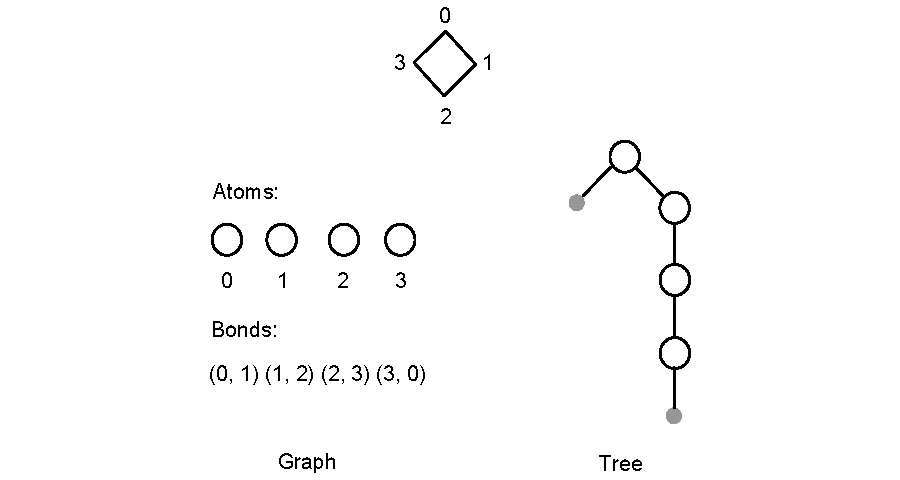
\includegraphics[width=6cm]{molecular-graph-vs-tree.pdf}
    \caption{Molecular Graph vs. Molecular Tree. The bonds in a molecular graph reference atoms indirectly through unique indexes (lower left). In contrast, a bond in a molecular tree defines its target atom inline (lower right). This increases the potential efficiency of trees over graphs for molecular representation. To simulate ring closure, a molecular tree introduces bridge nodes, as described later (solid grey circles).}
    \label{fig:molecular-graph-vs-tree}
\end{figure}

When discussing molecular trees, it's often useful to refer to \textit{node order} (Figure~\ref{fig:node-order}). An order is a property of a set that allows its members to be sorted through pairwise comparisons. Node order is the order in which the nodes of a molecular tree are added through depth-first construction. A node added before another node is said to \enquote{precede} it. A node added after another node is said to \enquote{succeed} it. In this way nodes can be prioritized. The root atom, uniquely lacking a parent, has highest priority because it precedes every other node. Similarly, a parent always precedes its children. Finally, the first child added to a given parent precedes all of its siblings. This relationship is transitive. If a node precedes (or succeeds) a sibling, then so do all of its descendants.

\begin{figure}
    \centering
    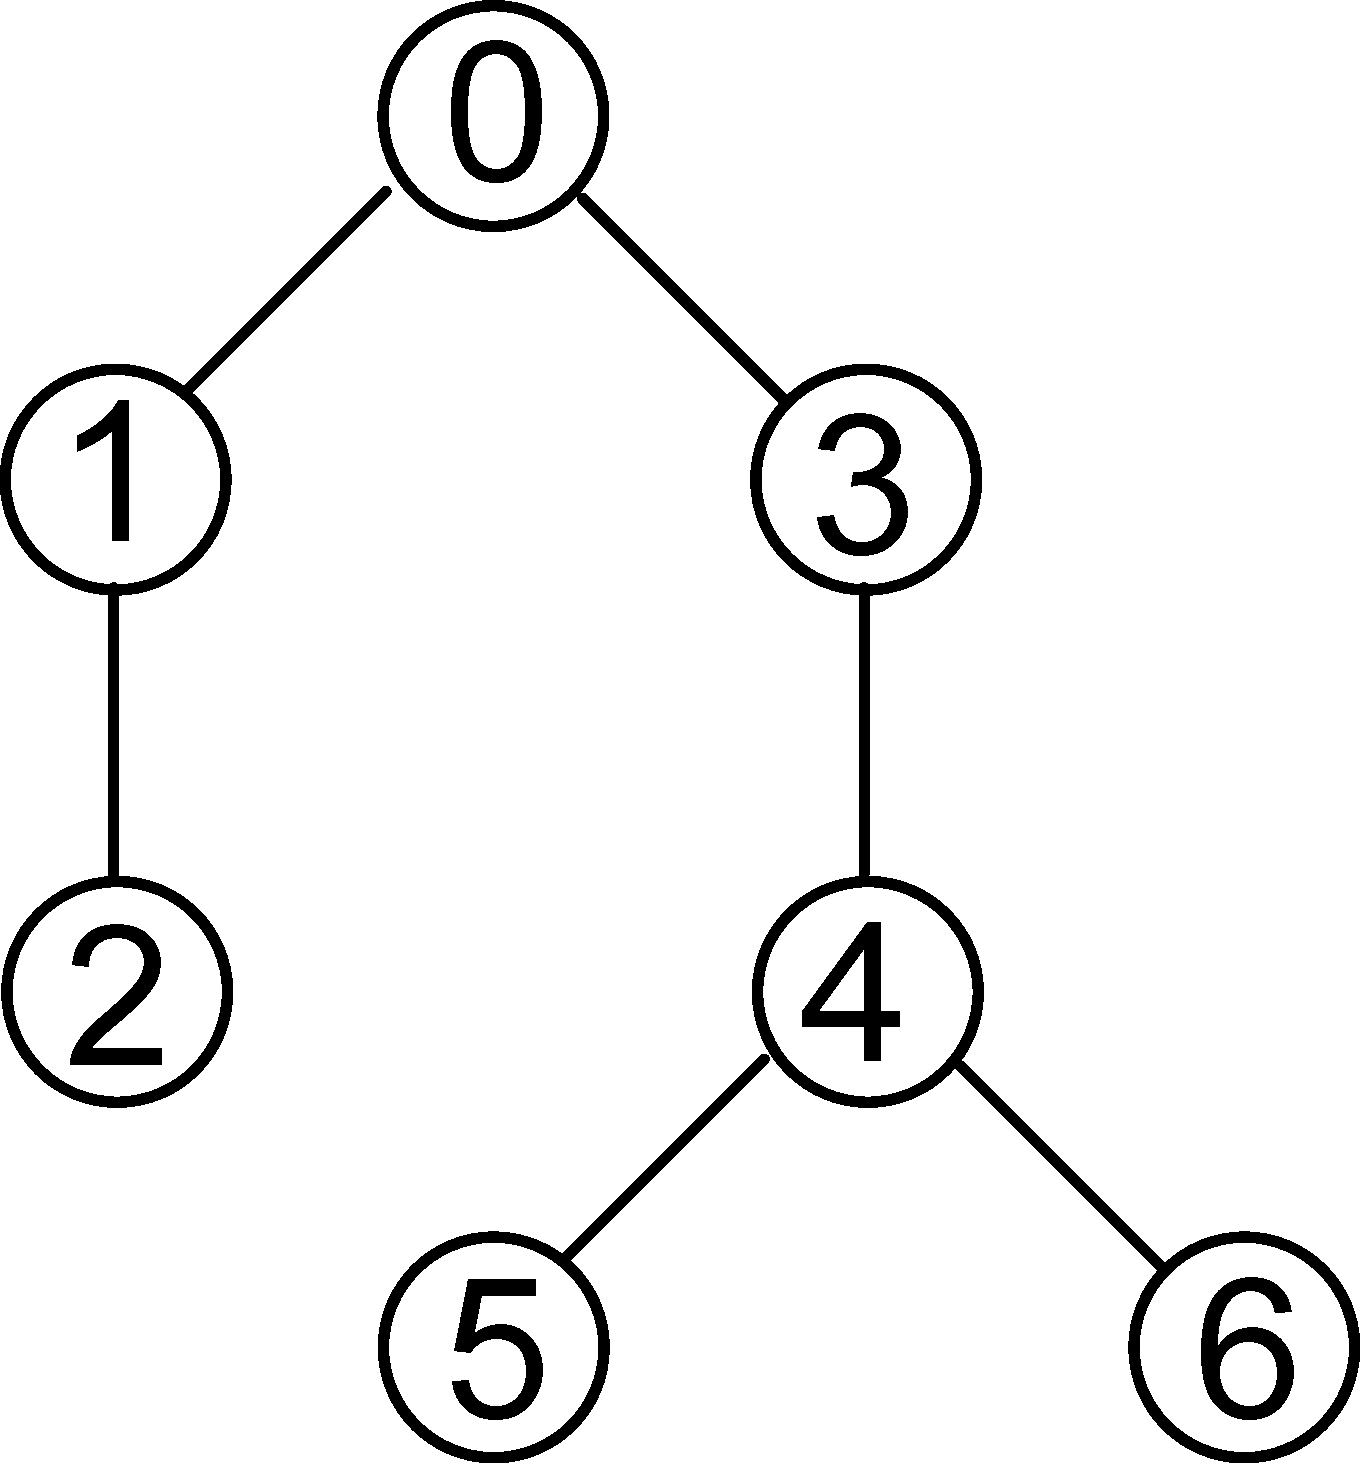
\includegraphics[width=2.5cm]{node-order.pdf}
    \caption{Node Order. Nodes in a molecular tree assume the order in which they were added through depth-first construction. Parents precede children, and children added first preceded those added later.}
    \label{fig:node-order}
\end{figure}

To support cycles and disconnected components, a molecular tree decouples connectivity from bonding (Figure~\ref{fig:nodes-and-edge-associations}). This means that nodes and edges don't generally map to atoms and bonds as they often do in molecular graphs. This indirection enables rings and disconnections to be encoded despite the fact that trees can contain no cycles or disconnected components.

Cycles are supported through \textit{bridges}. A bridge consists of two bond-node pairs that together represent one bond. One ach side of a bridge and atom connects to a bond, but the two atoms are not connected to each other. Instead, each atom is succeeded by a \textit{bridge node}. Unlike an atom, a bridge node has no children and so may not serve as the root of the tree. A bridge preserves the immediate atomic environment around each atom, allowing many of the same atomic computations possible in molecular graphs. Any bond, whether it closes a ring or not, can be represented as a bridge.

Each bridge node serves as a proxy to a \textit{referenced atom}. Should a bridge node be present during an operation that requires an atom, the referenced is used instead. Although a bridge node always succeeds its parent, the referenced atom may precede or succeed that parent.

Multiple molecules are supported through \textit{gaps}. A gap is an edge devoid of bonding. Gaps can be used whenever two or more molecules need to be encoded within the same molecular tree. Specific applications include ionic bonding and non-ionic complexes. However, no bonding relationship whatsoever is implied by the presence of a gap. In particular, the zero-order bond interpretation is excluded \cite{clark:2011}.

\begin{figure}
    \centering
    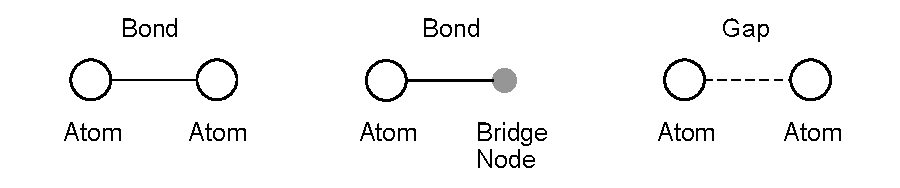
\includegraphics[width=4in]{node-and-edge-associations.pdf}
    \caption{Nodes and Edge Associations. Three node/edge associations are possible within a molecular tree. A parent atom can be connected to a child atom through a bond (left). A parent atom can also be connected to a child bridge node through a bond (center). Finally, an atom can be connected, without bonding, to a child atom through a gap (right).}
    \label{fig:nodes-and-edge-associations}
\end{figure}

Gaps and bridges decouple connectivity from bonding, but for opposite purposes. Whereas a gap connects two atoms without bonding them, a bridge creates a bond between two atoms without connecting them. These relationships can complicate the analysis of connectivity and bonding. For example, the atom succeeding a gap behaves in most situations as if it were a root. When tallying the bonds surrounding such an atom, only children are considered. Similar considerations apply when a gap succeeds an atom. Likewise, a bridge node behaves as if it were an atom in the sense that it connects to an atom through a bond. Nevertheless, a bridge node merely stands in for another atom found elsewhere in the tree. Bonding and connectivity analyses within molecular trees must therefore account for the possibility of connection-free bonds and bond-free connections. 

\subsection*{Atoms and Bonds}
\label{atoms-and-bonds}

Within a molecular tree, atoms and bonds play complementary roles. Atoms control nuclear particle counts, valence electron counts, and configuration. Bonds determine bonding electron counts and conformation. Constitution, configuration, and conformation are all influenced by the individual and collective behavior of atoms and bonds.

At the lowest level, atom and bond behavior are governed by their respective \textit{attributes}. An attribute is a key/value pair in which the key is a name composed of a character sequence and the value is constrained by a single, immutable \textit{type}. Types can be composed and decomposed, a feature supported by many programming languages.

\begin{table}
\begin{minipage}{\textwidth}
\renewcommand*\footnoterule{}
\caption{Primitives.}
\label{table:primitives}
\centering
\begin{tabular}{l l l l}
    \hline
    Name & Description & Notation & Values \\
    \hline
    \ttt{Option} & Optional value & \ttt{\{T\}} & \ttt{None}, $t$ \\
    \ttt{List} & Ordered list of values & \ttt{[T]} & $t_0, t_1, ... t_n$ \\
    \ttt{Range} & Bounded integer range & m..n & from \ttt{m} to \ttt{n}, excluding \ttt{n} \\
    \ttt{Boolean} & Boolean value & \ttt{?} & \ttt{true}, \ttt{false} \\
    \hline
\end{tabular}
\end{minipage}
\end{table}

Balsa types are composed of four \textit{primitives} (Table~\ref{table:primitives}). The first, \ttt{Option}, represents a value of a particular type that may either be present or absent. If not present, the special value \ttt{None} is used. A \ttt{List} is a possibly empty ordered collection of values of the same type. The \ttt{Range} type represents an integer value constrained by a lower inclusive bound (\ttt{m}) and an upper, exclusive bound (\ttt{n}). The \ttt{Boolean} type assumes one of two values: \ttt{true} or \ttt{false}.

An atom is composed of seven attributes (Table~\ref{table:atomic-attributes}). Default values are applied at the time of atom creation if no other values are used. The specific values assigned to an atom collectively define an \textit{atomic state}. 

\begin{table}
\caption{Atomic Attributes.}
\centering
\begin{tabular}{l L l l}
    \hline
    Attribute & Description & Type & Default \\
    \hline
    \ttt{element} & Elemental symbol & \ttt{\{Element\}} & \ttt{None} \\
    \ttt{isotope} & Mass number & \ttt{\{1..1000\}} & \ttt{None} \\
    \ttt{hydrogens} & Hydrogen count & \ttt{Implicit}, \ttt{0..10} & 0 \\
    \ttt{charge} & Formal charge & \ttt{-9..10} & 0 \\
    \ttt{selected} & Selection status & \ttt{?} & \ttt{false} \\
    \ttt{parity} & Configuration & \ttt{\{AtomParity\}} & \ttt{None} \\
    \ttt{edges} & Edges directed toward child nodes & \ttt{[Edge]} & \ttt{[]} \\
    \hline
\end{tabular}
\label{table:atomic-attributes}
\end{table}

The attributes \ttt{element} (\enquote{element}) and \ttt{isotope} (\enquote{isotope}) define atomic number and neutron count, respectively. Elements are selected from a subset of those approved by IUPAC \cite{periodicTable} (Figure~\ref{fig:periodic-table}). An atom whose element is unknown must have an \ttt{element} attribute equal to \ttt{None}. The \ttt{isotope} attribute is an optional integer value representing an atom's nuclear mass number, defined as the sum of proton and neutron count. Setting the \ttt{isotope} property to \ttt{None} means that the element's isotopic composition equals natural abundance. Otherwise, the lower bound of the value of \ttt{isotope} is one. This lower limit allows for physically nonsensical states such as atoms of negative implied neutron count (e.g., carbon-5). Implementations may reject such atomic states as invalid.

\begin{figure}
    \centering
    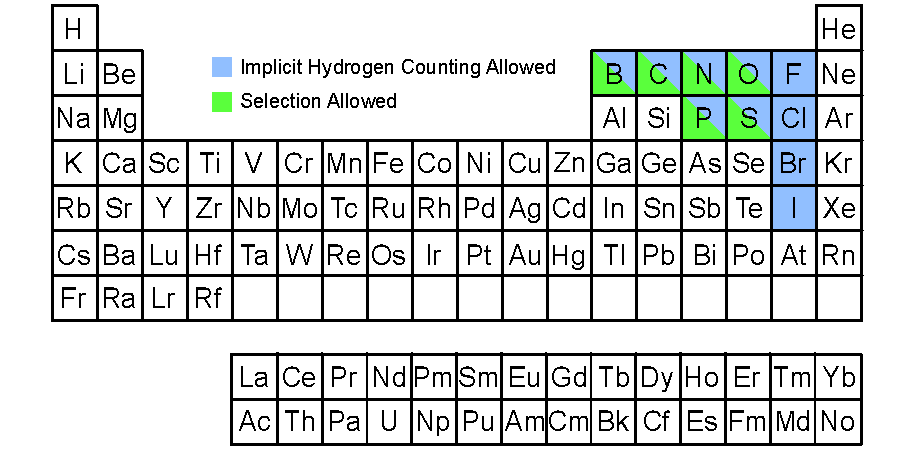
\includegraphics[width=4in]{periodic-table.pdf}
    \caption{Elements. Available chemical elements and their allowed roles. Not all IUPAC-approved elements are available. Hydrogen counts of atoms associated with elements on blue background can be computed algorithmically. Atoms associated with elements on green background can be selected.}
    \label{fig:periodic-table}
\end{figure}

The \ttt{hydrogens} attribute sets an atom's mode of \textit{hydrogen suppression}. Hydrogen suppression replaces an atomic hydrogen of natural isotopic abundance and its associated bond with an integer tally associated with the parent atom. Even so, a suppressed hydrogen and its bond are understood to be present. The high relative abundance and regular bonding of hydrogen atoms makes hydrogen suppression an effective technique for increasing information density. Two mutually-exclusive types of suppressed hydrogen are supported: \textit{virtual hydrogen} and \textit{implicit hydrogen}.

A virtual hydrogen is one that appears as an integer unit contribution associated with the parent atom. For example, methane can be represented using five atoms and four bonds. But methane can also be represented as a single atom whose \ttt{hydrogens} attribute equals four. Virtual hydrogen count defaults to zero, and may be set to a maximum value of nine. By default, atoms use virtual hydrogen counting.

An implicit hydrogen is similar to a virtual hydrogen in that both the hydrogen atom and bond have been replaced with a tally. Unlike a virtual hydrogen, however, this tally is not present as an attribute on the parent atom but rather as a computation. Setting the \ttt{hydrogens} attribute to \ttt{Implicit} activates implicit hydrogen counting. However, not all atoms are eligible to do so (see: \nameref{computing-implicit-hydrogen-count}).

The \ttt{charge} (\enquote{charge}) and \ttt{selected} (\enquote{selected}) attributes determine valence electron count (see: \nameref{electron-counting}). Charge refers formal charge, or the difference between the valence electron count of the element and the sum of bonding and nonbonding electrons of the bound atom. By default, an atom is assigned a charge of zero. Minimum and maximum values for charge are -9 and +9, respectively. The \ttt{selected} attribute adjusts an atom's selection status. Selecting an atom allows it to participate in extended bonding (see: \nameref{delocalization-subgraph}).

Configuration is determined by the \ttt{parity} attribute (\enquote{atom parity}). The type of this value, \ttt{AtomParity} is an enumeration supporting two values: \ttt{Clockwise} and \ttt{Counterclockwise} (Table~\ref{table:atom-parity-variants}). The interpretation and encoding of atom parity will be described in detail later (see: \nameref{configuration}).

\begin{table}
\caption{Atom Parity Variants.}
\centering
\begin{tabular}{l l}
    \hline
    Variant & Description  \\
    \hline
    \ttt{Clockwise} & Configuration runs with node order. \\
    \ttt{Counterclockwise} & Configuration runs against node order. \\
    \hline
\end{tabular}
\label{table:atom-parity-variants}
\end{table}

The \ttt{edges} ("edges") attribute is a possibly empty ordered list of edges associated with an atom. As noted in the previous section, an edge may represent either a bond or a gap (Table~\ref{table:edge-variants}). The mere presence of an edge does not guarantee a bonding relationship.

\begin{table}
\caption{Edge Variants.}
\centering
\begin{tabular}{l l}
    \hline
    Variant & Description  \\
    \hline
    \ttt{Bond} & A bonding and connectivity relationship. \\
    \ttt{Gap} & A connectivity relationship only. \\
    \hline
\end{tabular}
\label{table:edge-variants}
\end{table}

Not all atomic states are valid. Implementations must ensure either the impossibility of creating an invalid state, or an error condition in the event that one is created. Atomic state is restricted in the following two ways:

\begin{enumerate}
    \item{If implicit hydrogen counting is used, default values of isotope, charge, and parity must also be used. Implicit hydrogen counting is only supported for elements in the list: B; C, N; O; P; S; F; Cl; Br; or I.}
    \item{A selected atom must use one of the following five elements: B; C; N; O; P; or S.}
\end{enumerate}

A bond is composed of four attributes (Table~\ref{table:bond-attributes}). The \ttt{order} attribute (\enquote{order}) represents the concept of formal bond order, or the number of bonding electrons divided by two. A bond's order may only assume the values one, two, or three. The \ttt{elided} attribute (\enquote{elided}) allows a bond to be omitted during serialization and participate in extended bonding. The \ttt{direction} attribute (\enquote{direction}) is used with other information to conformationally restrict a bond. The two allowed variants for \ttt{Direction}, \ttt{Up} and \ttt{Down}, will be described in detail later (see: \nameref{conformation}). The \ttt{target} attribute identifies the child node at which the bond is directed (Table~\ref{table:target-variants}).

\begin{table}
\caption{Bond Attributes.}
\centering
\begin{tabular}{l p{3.6cm} l l}
    \hline
    Attribute & Description & Type & Default \\
    \hline
    \ttt{order} & Formal bond order & \ttt{1..4} & 1 \\
    \ttt{elided} & Elision status & \ttt{boolean} & \ttt{false} \\
    \ttt{direction} & Partial conformational parity & \ttt{\{Direction\}} & \ttt{None} \\
    \ttt{target} & An atom or bridge node & \ttt{Target} & - \\
    \hline
\end{tabular}
\label{table:bond-attributes}
\end{table}

\begin{table}
\caption{Target Variants.}
\centering
\begin{tabular}{l p{6.6cm}}
    \hline
    Variant & Description \\
    \hline
    \ttt{Atom} & A parent and child atom are bound. \\
    \tt{Bridge} & A parent atom and bridge node are bound. \\
    \hline
\end{tabular}
\label{table:target-variants}
\end{table}

As with atomic state, not all bond states are valid. The following restrictions apply:

\begin{enumerate}
    \item{An elided bond must have an order of one and default direction.}
    \item{A bond with a non-default direction must have an order of one.}
\end{enumerate}

The atom and bond attributes defined here will be referenced throughout this paper as a way to connect syntax and semantics. Implementations may, of course, use any suitable internal data model. They must, however, ensure that any internal data model is consistent with the one provided here.

\subsection*{Electron Counting}
\label{electron-counting}

A molecular tree explicitly encodes the presence of protons and neutrons through the atomic attributes \ttt{element} and \ttt{isotope}, respectively. The presence of electrons, in contrast, is merely implied. The principles of charge and mass conservation nevertheless require a method to determine explicit electron counts. This is possible through \textit{electron counting}. 

Electron counting in Balsa is based on the well-known \textit{valence bond model} (VB Model)~\cite{lewis:1916}. This model assumes that a bond spans exactly two atoms and is associated with a nonzero, positive, and even number of electrons. These electrons are drawn in equal quantities from each atom's set of valence electrons. A single bond draws one electron from each atom (two total), a double bond two (four total), and a triple bond three (six total). The electron count of an atom whose \ttt{element} attribute equals \ttt{None} is always zero. Bonding to such an atom adds the required number of electrons directly to the bond.

Electrons are counted as follows (Figure~\ref{fig:electron-counting}). A molecular tree starts as a single root atom. The electron count of this atom equals the difference between proton count (atomic number) and charge. Adding a bond is a three-step process. First, a child atom is constructed with an electron count determined in the same way as the root atom. Next, the child atom and the bond are added to the molecular tree. Finally, the electron counts of each atom and the bond are updated. If parent and child are connected through a gap edge, no electrons are deducted from either atom. Should a parent atom be bound to a child bridge node, then the electron count of the referenced atom is not changed.

\begin{figure}
    \centering
    
\includegraphics[width=\columnwidth]{electron-counting.pdf}
    \caption{Electron Counting. A root atom and its child are added to a tree (left). Next, a bond is added (center). Finally, the appropriate electron count is deducted from each atom and added to the bond (right).}
    \label{fig:electron-counting}
\end{figure}

Whereas negative bond order is disallowed by definition, Balsa places no restrictions on \textit{hypervalence}. Hypervalence occurs when an atom undergoes enough bonding operations to leave it with a negative implied valence electron count. Consider lithium, which possesses one valence electron. Formation of one single bond leaves lithium with zero implied valence electrons. Application of a second bond formation leaves lithium with a zero charge and an implied valence electron count of -1. Such an arrangement may be physically meaningless, but Balsa explicitly supports it. Software using Balsa may or may not reject such species on semantic grounds.

\subsection*{Delocalization Subgraph}
\label{delocalization-subgraph}

A molecular representation based solely on the valence bond model can yield artifacts resulting from \textit{delocalization induced molecular equality} (DIME, Figure~\ref{fig:dime}). DIME arises when a given molecule can be represented by two forms, each differing from the other only in double bond placement. DIME is sometimes referred to as \enquote{resonance} or \enquote{aromaticity,} but those terms are avoided here due to their ambiguity~\cite{randic:2018,kerber:2006}.

\begin{figure}
    \centering
    
\includegraphics[width=2in]{dime.pdf}
    \caption{Delocalization-induced molecular equality (DIME). Two chemically equivalent molecular representations differ only due to delocalization.}
    \label{fig:dime}
\end{figure}

The main problem with DIME is its interference with \textit{canonicalization}, or the selection of a single molecular representation among many alternatives. The presence of multiple equivalent molecular forms differing only in electron delocalization complicates the formulation of selection rules and invariants, which must be adapted to account for the artificial asymmetry.

To eliminate DIME and thereby streamline canonicalization, each molecular tree is augmented with a \textit{delocalization subgraph} (DS). A DS is a possibly empty node-induced subgraph over a molecular tree. The membership of a DS will typically be drawn from the set of atoms and bonds that participate in DIME within a given molecular tree.

Membership of a DS is determined as follows. An atom is added to the DS by setting its \ttt{selected} attribute to \ttt{true} through a process called \textit{selection}. As noted previously (see: \nameref{atoms-and-bonds}), only some atomic states are compatible with selection. An edge will be added to the DS if both of the atoms it spans are selected and the bond itself is elided. This allows arbitrary bonds between selected atoms to be excluded from the DS. If a bond's target is a bridge node, the corresponding edge will be added to the DS if both the parent atom and the equivalent target atom are selected.

\begin{figure}
    \centering
    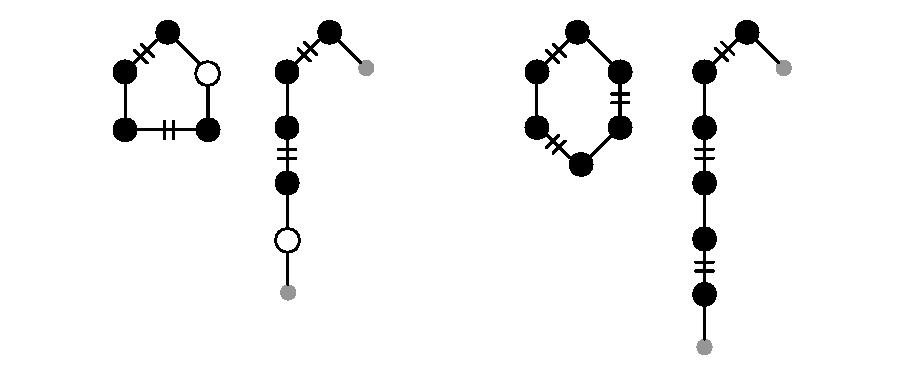
\includegraphics[width=\columnwidth]{matching.pdf}
    \caption{Perfect Matching. A matching is a subgraph in which all nodes have degree one. A perfect matching contains all of the nodes of its parent. Nodes and edges of a matching are noted with black circles and hashed lines, respectively. The five-membered cycle on the left has no perfect matching. Such graphs are not valid delocalization subgraphs. The six-membered cycle on the right has a perfect matching, and would be a valid delocalization subgraph. Either graph or tree representation can be used to construct a perfect matching, but published algorithms use graphs.}
    \label{fig:perfect-matching}
\end{figure}

A non-empty DS must possess a \textit{perfect matching} (Figure~\ref{fig:perfect-matching}). A matching is a subgraph in which no two edges share a common node. Equivalently, a matching is a subgraph in which all nodes have degree one. A perfect matching includes every node present in the parent graph. Every atom added to a DS must therefore become part of its perfect matching.

A filled DS can be emptied through a two-step process of \textit{deselection} (Figure~\ref{fig:selection-and-deselection}). First, a perfect matching over the DS is found. Next, the elided bond corresponding to each matched edge is replaced by a double bond. Because the presence of a filled DS implies a perfect matching over it, kekulization always succeeds. A widely-used algorithm for matching, the Edmunds \enquote{blossom algorithm,} has a time complexity of $O(|E||V|^2)$, where $|E|$ is the number of edges and $|V|$ is the number of nodes~\cite{edmonds:1965}. Although more efficient algorithms are known, they are either much more difficult to implement or lack generality.

\begin{figure}
    \centering
    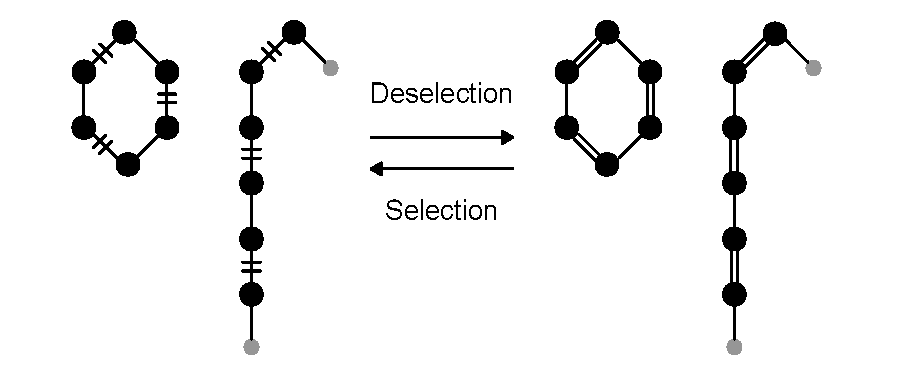
\includegraphics[width=\columnwidth]{selection-and-deselection.pdf}
    \caption{Deselection and Selection. Deselection unsets the atomic selected flag (open circle) with simultaneous promotion of matching bonds. Selection sets the atomic selected flag (closed circle) with simultaneous demotion of intervening single and double bonds to elided bonds.}
    \label{fig:selection-and-deselection}
\end{figure}

The opposite operation can be accomplished with a \textit{selection algorithm}. A selection algorithm selects two or more atoms, thereby adding them to the DS. The only requirement for a selection algorithm is that the resulting DS must have a perfect matching. Depending on the application, other criteria may be applied. For example, a selection algorithm may restrict candidate atoms to those found in cycles. Electron-counting techniques may also be introduced to approximate the chemical concept of \enquote{aromaticity.} Elision of the single bonds to be added to the DS completes the process.

Selection is nothing more than an alternative to explicit bond order encoding. No other properties whatsoever are conferred to selected atoms. The members of a DS may be assigned the labels \enquote{aromatic,} \enquote{antiaromatic,} \enquote{non-aromatic,} or any number of other designations by downstream applications. Two encodings differing only in the presence of a DS should be considered equivalent. Balsa itself provides no guidance at all about whether or not selectable atoms should be selected, although individuals and organizations may do so.

\subsection*{Valence and Subvalence}
\label{valence-and-subvalence}

To support implicit hydrogen counting, Balsa uses the concept of \textit{valence}. Valence is a non-negative integer computed as the sum of bond orders at a given atom. Single and elided bonds contribute one to the tally, double bonds two, and triple bonds three. Each virtual hydrogen contributes one. For example, the valence of a methyl carbon having three virtual hydrogens and a hydrogen neighbor is four. The valence of an acetaldehyde oxygen atom is two. And so on.

Some elements are associated with one or more \textit{default valences} (Table~\ref{table:default-valences}). A default valence is the number of hydrogens that can be attached to an isolated, fully-saturated atom using the corresponding element. For example, the default valence for a carbon-bearing atom is 4. This means that a fully saturated atom of carbon will have four hydrogens. Likewise, a fully-saturated atom of oxygen will have two hydrogens. Some elements such as nitrogen are associated with multiple default valences. In these cases, multiple saturated forms are possible. For example, nitrogen has the default valences three and five. Both ammonia (NH\textsubscript{3}) and nitrogen pentahydride (NH\textsubscript{5}) are therefore fully saturated forms of nitrogen according to Table~\ref{table:default-valences}.

\begin{table}
    \caption{Default Valences.}
    \centering
    \begin{tabular}{l l}
        \hline
        Element & Valences \\
        \hline
        B & 3 \\
        C & 4 \\
        N & 3,5 \\
        O & 2 \\
        F & 1 \\
        P & 3,5 \\
        S & 2,4,6 \\
        Cl & 1 \\
        Br & 1 \\
        I & 1 \\
        \hline
    \end{tabular}
    \label{table:default-valences}
\end{table}

Given an atom whose element has one or more default valences, \textit{subvalence} can be computed (Algorithm~\ref{algorithm:subvalence}). Subvalence is the number of hydrogens that can be added to an atom without exceeding the lowest possible default valence. If no suitable default valence exists, then subvalence equals zero. This computation can be expressed algorithmically (Algorithm~\ref{algorithm:subvalence}). First, the atom's valence is computed. Next, the ordered list of default valences of the atom's element is found. For each default valence, the difference between it and the valence is compute. If this differences is positive, it is returned as the subvalence. If no suitable default valence is found, zero is returned. The subvalence of an atom whose element has no default valences (i.e., no listing in Table~\ref{table:default-valences}) is zero. For example, an iron atom always has a subvalence of zero, regardless of how it is bonded.

\begin{algorithm}
    \SetKwInOut{Input}{input}
    \SetKwInOut{Output}{output}
    \SetKwFunction{BondOrderSum}{BondOrderSum}
    \SetKwFunction{TargetValences}{TargetValences}
    \caption{Computing subvalence.}
    \label{algorithm:subvalence}
    
    \Input{An atom $a$ with one or more default valences}
    \Output{The subvalence of $a$}
    \Begin{
      $v \leftarrow$ Valence($a$)\;
      $T \leftarrow$ DefaultValences($a$)\;
      \For{$t \in T$}{
        $d \leftarrow t-v$\;
        \If{$d >= 0$}{
          \Return{$d$}\;
        }
      }
      \Return{$0$}\;
    }
\end{algorithm}

For a representative subvalence computation, consider an isolated nitrogen atom without virtual hydrogens. The atom's bond order sum is zero. Its default valences are 3 and 5. The difference is found to be three ($3 - 0$). Therefore, the subvalence of this atom is three.

The carbonyl carbon atom of acetaldehyde illustrates the effects of substitution and multiple bonding. Bond order sum is three (2 + 1). From Table~\ref{table:default-valences}, default valence is four. Subtracting bond order sum from default valence yields one ($4 - 3$), which is returned as the atom's subvalence.

The phosphorous atom in phosphorous acid (H\textsubscript{3}PO\textsubscript{3}) illustrates the use of Algorithm \ref{algorithm:subvalence} for atoms with multiple target valences. Bond order sum is four ($2 + 1 + 1$). The first default valence is 3, but subtracting valence from that value yields a negative number ($3 - 4$). Continuing to the next default valence, five, a difference of 1 is obtained. Therefore, the subvalence of the phosphorous-bearing atom is reported as one.

The valence of some atoms exceeds the largest default valence. In these cases, subvalence is reported as zero. Consider sodium perchlorate (NaClO\textsubscript{4}). The chlorine atom has a bond order sum of seven ($2 + 2 + 2 + 1$). From Table~\ref{table:default-valences}, the only default valence for chlorine is one. Subtracting seven yields a negative number (-6). Therefore, the subvalence is reported as zero.

\subsection*{Computing Implicit Hydrogen Count}
\label{computing-implicit-hydrogen-count}

An atom whose \ttt{hydrogens} attribute equals \ttt{Implicit} signals that its hydrogens must be counted algorithmically. The exact algorithm depends on the value of the atoms's \ttt{selected} attribute (Figure~\ref{fig:implicit-hydrogen-count}).

For an unselected atom, implicit hydrogen count equals subvalence. For example, an oxygen atom with one single bond has an implicit hydrogen count of one because subvalence is one ($2 - 1$). Similarly, an oxygen atom with two singly-bonded neighbors has an implicit hydrogen count of zero ($2 - 2$).

For a selected atom, implicit hydrogen count equals subvalence minus one. This subtraction accounts for the extra valence implied by the atom's membership in the delocalization subgraph. Consider a selected carbon atom in benzene with a \ttt{hydrogens} attribute of \ttt{Implicit}. Subvalence equals two ($4 - 2$), so implicit hydrogen count equals one ($2 - 1$). Likewise, the subvalence of a selected nitrogen atom in pyridine equals one ($3 - 2$) so implicit hydrogen count equals zero ($1 - 1$). Stated differently, the calculation ensures that an atom's implicit hydrogen count is identical before and after deselection.

If the subvalence of a selected atom equals zero, then an implicit hydrogen count of zero is reported. The meaning of such an atomic state may seem suspect because an atom without a free valence can not perform the required promotion of a single bond during deselection. As will be explained in detail later (Pruning), this situation can arise for reasons of convenience or tradition. Returning zero avoids miscalculation of the implicit hydrogen count.

An atom's implicit hydrogen count may or may not correlate with chemical intuition or experimental data. Consider the phosphorous-bearing atom of hypophosphorous acid (HOP(O)H\textsubscript{2}). We might expect the implicit hydrogen count to equal the experimentally-determined hydrogen count (2). However, the subvalence for the phosphorous atom is found to be three ($2 + 1 - 3$). The implicit hydrogen count is therefore zero ($3 - 3$) rather than the expected two. To represent this atom and other like it, virtual hydrogens must be used.

\begin{figure}
    \centering
    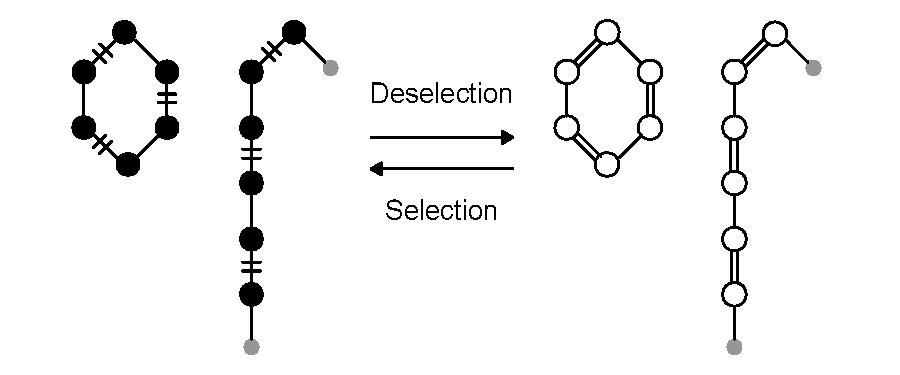
\includegraphics[width=\columnwidth]{implicit-hydrogen-count.pdf}
    \caption{Implicit hydrogen count. The number of hydrogens is computed algorithmically. For unselected atoms (top left, top right, bottom right), implicit hydrogen count equals subvalence. For selected atoms (bottom left), implicit hydrogen count equals subvalence minus one. The hydrogen count for an atom whose element lacks at least one default valence can not be determined algorithmically.}
    \label{fig:implicit-hydrogen-count}
\end{figure}

\subsection*{Conformation}
\label{conformation}

Restricted rotation about a bond leads to conformational isomers (\enquote{conformers}). When the bond in question is a double bond, two conformers result. They can be distinguished through \textit{partial parity bonds} (PPBs). As the name implies, a PPB encodes some of the parity information characterizing a conformationally restricted double bond. Reconstruction of the full parity requires the double bond itself and at least one flanking PPB at each terminal.

\begin{figure}
    \centering
    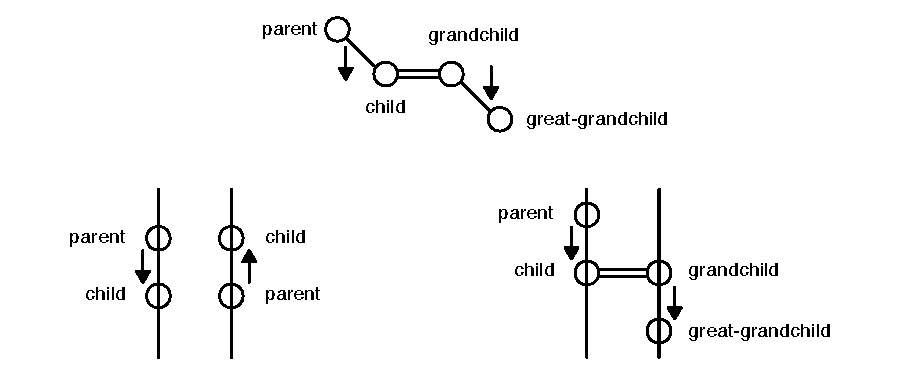
\includegraphics[width=\columnwidth]{partial-parity-bond.pdf}
    \caption{Partial parity bond (PPB). Double bond conformational parity is distributed over at least three bonds. A minimal assembly contains a double bond, two flanking PPBs (marked with upward- or downward-facing arrows), and associated nodes (top). To determine 2D orientation, parent and child are arranged on a vertical axis with parent above child for a bond direction of Down, and child above parent for a bond direction of Up (bottom-left). A complete diagram places parent, child, grandchild and great-grandchild (bottom right).}
    \label{fig:partial-parity-bonds}
\end{figure}

A PPB is designated by setting its \ttt{direction} attribute to a non-default variant (\ttt{Up} or \ttt{Down}). The names of these variants refer to a two-dimensional geometrical model in which a parent atom and its child are placed along a vertical axis. If the child lies above the parent, the \ttt{Up} variant is used. If the child lies below the parent, the \ttt{Down} variant is used.

The parity of a double bond is determined by the relative direction of the PPBs neighboring it (Figure~\ref{fig:partial-parity-bonds}). First, the parent atom is identified. This atom has the lowest order in the assembly, meaning that it was added first to the molecular tree. The parent is placed on a vertical axis. Bonds from the parent atom are then iterated. If a PPB is found, its child atom is placed above the parent for a direction of \ttt{Up} or below the parent for a direction of \ttt{Down}. The child's bonds are then iterated in order. Should an additional PPB be found, its direction must match that of the bond between parent and child. Otherwise an error must be reported. An error must also be reported if more than two PPBs are present. If a double bond is found, its target, a grandchild, is placed to the right of the parent. The bonds of the grandchild are then iterated in order. The target of the first PPB, a great-grandchild, is placed as before, above the grandchild if the direction is \ttt{Up}, or below if the direction is \ttt{Down}. If a second PPB is present, it must have a direction opposite the first. Otherwise an error must be reported.

The placement of parent, child, grandchild, and great-grandchild will yield one of two parities (Figure~\ref{fig:ppb-placement}). For convenience and to avoid confusion, these parities are given the labels  \textit{syn} (vertical lines both lie above or below the double bond) and \textit{anti} (vertical lines lie on opposite sides of the double bond).

\begin{figure}
    \centering
    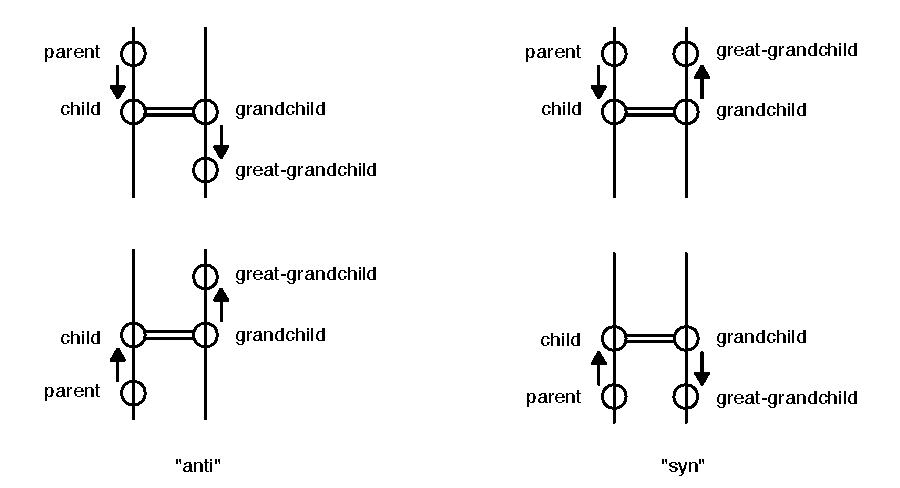
\includegraphics[width=\columnwidth]{partial-parity-bond-placement.pdf}
    \caption{Partial Parity Bond Placement. Two unique modes of PPB placement are \textit{syn} and \textit{anti} (left and right, respectively). Within each mode is an equivalent pair of PPB pairs.}
    \label{fig:ppb-placement}
\end{figure}

To illustrate, consider the placement for (\textit{E})-2-butene. The parent atom, a methyl group, is placed on a vertical axis. Bonds are iterated and a PPB with a direction of \ttt{Down} is found. The child attached to the bond is therefore placed below the parent. Iterating the child's bonds reveals one bond of order two. The atom attached to it is placed to the right of the previous child. Bonds are again iterated, revealing a PPB whose direction is \ttt{Down}. The atom attached to this bond is then placed below its parent. The completed diagram reveals the \textit{anti} conformation.

The same procedure works in reverse when encoding the \ttt{direction} attribute (Figure~\ref{fig:assigning-ppb}). 2-butene having the \textit{anti} conformation is modeled using a diagram whose left- and right-hand sides point downward and upward, respectively. The parent atom, a primary carbon, is identified. It is bonded to one neighbor through a PPB. To match the diagram, a direction of \ttt{Up} is assigned. The child atom is attached to its own child through a double bond. Finally, the grandchild is attached to its own child through a PPB whose direction is consistent with the diagram. A direction of \ttt{Up} is therefore assigned.

\begin{figure}
    \centering
    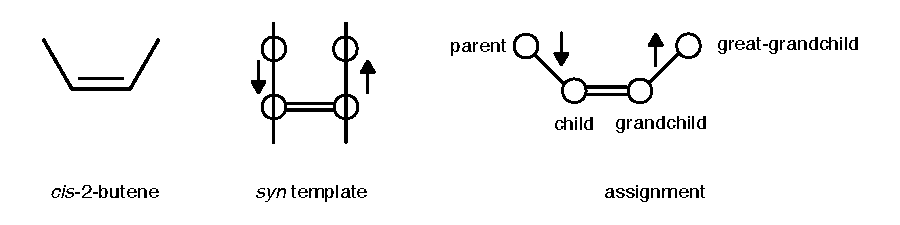
\includegraphics[width=\columnwidth]{assigning-ppbs.pdf}
    \caption{Assigning partial parity bonds to \textit{cis}-2-butene.}
    \label{fig:assigning-ppb}
\end{figure}

Spreading conformational parity over more than one bond in this way means that several error states are possible (Figure~\ref{fig:bond-error-states}):

\begin{itemize}
    \item{Overspecification. Two children are forced into the same direction along an axis.}
    \item{Underspecification. A required PPB is missing.}
    \item{ Misspecification. A PPB is used between atoms, neither of which connects to a double bond.}
\end{itemize}

An error must be reported should any of these states be encountered. Note that it is possible for a conformation to be both overspecified on one side and underspecified on the other.

\begin{figure}
    \centering
    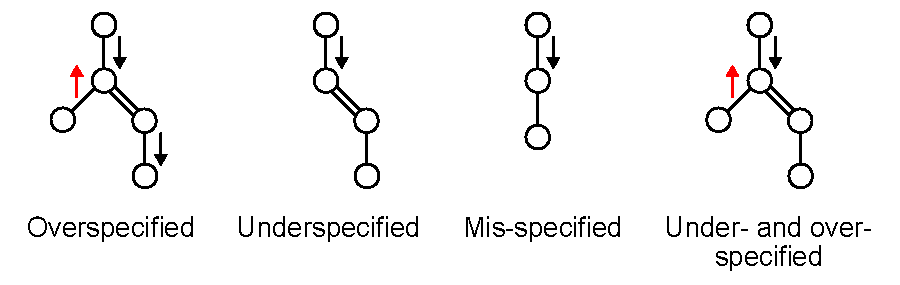
\includegraphics[width=\columnwidth]{ppb-error-states.pdf}
    \caption{PPB error states. Because conformational descriptions are defined over three or more bonds, a variety of error states are possible.}
    \label{fig:bond-error-states}
\end{figure}

An exception to the underspecification rule applies in the case of conjugated polyenes (Figure~\ref{fig:bond-error-state-exceptions}). Here, a PPB may run from parent to child but not from grandchild to great-grandchild. No error is reported in such a case and the conformation of the terminal double bond remains undefined.

\begin{figure}
    \centering
    
\includegraphics[width=\columnwidth]{ppb-error-state-exception.pdf}
    \caption{Error state exceptions. Conjugated dienes sharing a common PPB can lead to exceptional cases. The direction of the rightmost bond does not need to be set.}
    \label{fig:bond-error-state-exceptions}
\end{figure}

The presence of a bridge node within a PPB complicates the assignment of direction (Figure~\ref{fig:bridged-ppb-bond}). A bridge node has no children and therefore can never be a parent. At the same time, a bond always points from parent to child. This means that a bridged PPB yields a pair of bonds with opposite directions. The first (or "left") bond, has the direction that would result from a direct bond to an atomic child. The second (or "right") bond has the opposite direction.

\begin{figure}
    \centering
    
\includegraphics[width=\columnwidth]{bridged-ppb-bond.pdf}
    \caption{Bridged PPB Bond. A bridge across a PPB yields two bonds of opposite direction (right).}
    \label{fig:bridged-ppb-bond}
\end{figure}

Cyclic conjugated polyenes present special challenges to the use of PPBs, as exemplified by cyclooctatetraene (Figure~\ref{fig:cyclooctatetraene}). Although the (\textit{anti}, \textit{anti}, \textit{anti}, \textit{anti}) conformation is expressable, the (\textit{syn}, \textit{anti}, \textit{anti}, \textit{anti}) conformation is not. This problem arises because the conformation for two different double bonds is set by the same PPB.

\begin{figure}
    \centering
    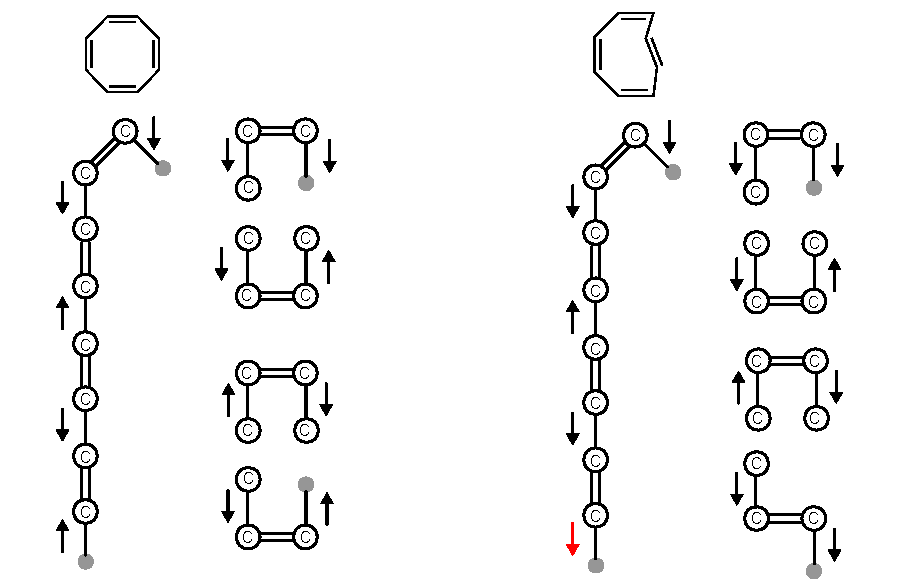
\includegraphics[width=\columnwidth]{cyclooctatetraene.pdf}
    \caption{Cyclooctatetraene. The all-(\textit{Z}) conformation is expressable (left), but the (\textit{Z},\textit{Z},\textit{Z},\textit{E}) conformation is not (right). Although the local conformations for the latter are all valid, the global conformation introduces a conflict, the direction marked in red.}
    \label{fig:cyclooctatetraene}
\end{figure}

\subsection*{Configuration}
\label{configuration}

Balsa limits configuration to the special case of an atom with exactly four substituents placed at the vertices of a tetrahedron. Here, \enquote{substituent} means an atomic neighbor or virtual hydrogen. Lone electron pairs are not considered to be substituents.

The configuration about an atom can specified through its \ttt{parity} attribute. This attribute, together with a general convention, determine the relative three-dimensional positioning of substituents about a central atom (Figure~\ref{fig:atom-parity}). First, the parent of the central atom is identified. Then the frame of reference is shifted by sighting down the bond from the central atom's parent to the central atom. An equilateral triangle is then inscribed about the central atom. The bonds from the central atom are then iterated in order. If the parity of the central atom equals \ttt{Clockwise}, the child atoms attached through each bond are placed around the triangle in clockwise order. Otherwise the children are arranged in counterclockwise order.

\begin{figure}
    \centering
    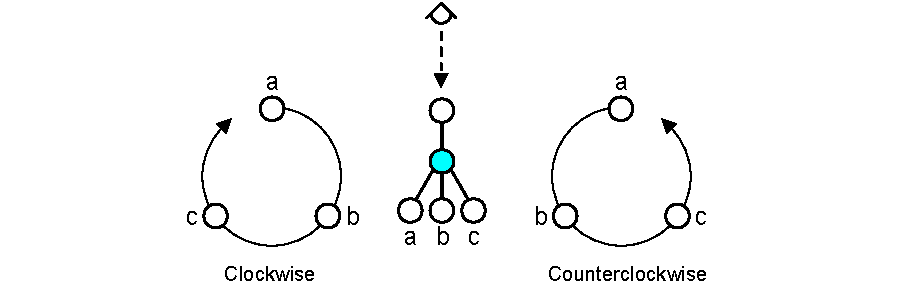
\includegraphics[width=\columnwidth]{atom-parity.pdf}
    \caption{Atom parity. Four substituents surround a central atom with non-default atom parity (cyan). Sighting from the parent to the central atom, its children (a, b, and c) follow either a clockwise or counterclockwise pattern when iterated in order.}
    \label{fig:atom-parity}
\end{figure}

The convention is modified for atoms bearing one virtual hydrogen and three atomic substituents (Figure~\ref{fig:atom-parity-suppressed-hydrogen}). The implied bond to the virtual hydrogen is considered to precede the others. Sighting down this bond, the central atom's parent is placed on the triangle at an arbitrary position. Children are then iterated counterclockwise or clockwise relative to it.

\begin{figure}
    \centering
    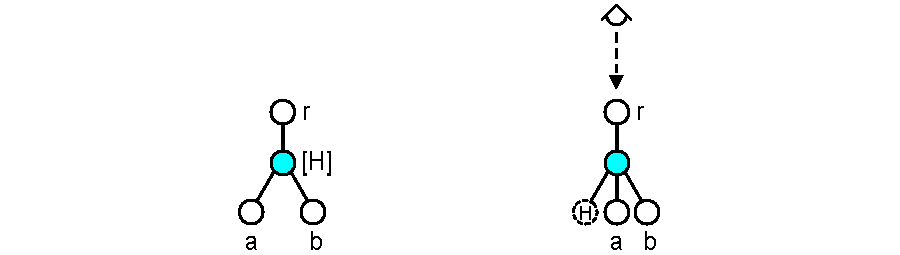
\includegraphics[width=\columnwidth]{atom-parity-suppressed-hydrogen.pdf}
    \caption{Atom parity with one virtual hydrogen. The central atom (cyan) has a virtual hydrogen (left). In this case, the virtual hydrogen assumes the role of root atom (right). The former root atom (r) then assumes the role of the first child,  and analysis continues as before.}
    \label{fig:atom-parity-suppressed-hydrogen}
\end{figure}

One additional modification applies to a central atom without a parent. The frame of reference is shifted to sight along the direction of the first child. The remaining children are then placed around the triangle in either counterclockwise or clockwise order according to the value of the central atom's \ttt{parity} attribute. If a central root atom bears a virtual hydrogen, it is considered to be the first child.

A central atom whose parity attribute assumes a non-default value must have either four bonds if no virtual hydrogens are present, or three bonds if one virtual hydrogen is present. Some topologies might appear to be similar enough that the \ttt{parity} attribute can be used, but they all must be reported as errors (Figure~\ref{fig:invalid-atom-parity}). Examples include the central atom of allenes and other odd cumulenes, and the sulfur atom of sulfoxides where the lone pair is misconstrued as a substituent.

\begin{figure}
    \centering
    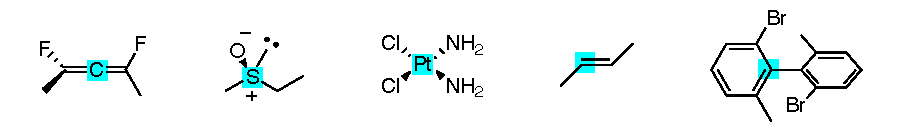
\includegraphics[width=\columnwidth]{invalid-atom-parity.pdf}
    \caption{Invalid uses of atom parity. Only configuration about tetrasubstituted, tetrahedral atoms is supported. The marked atoms (cyan background) lack four substituents, tetrahedral geometry, or both. Assigning a non-default atom parity to any of them would be an error.}
    \label{fig:invalid-atom-parity}
\end{figure}

Configurational descriptors may be assigned without regard to bond order. In other words, single, double, triple, and PPBs can all be present. The only requirement that must be satisfied by a central atom is an atomic neighbor count of four, or three when a virtual hydrogen is present.

It is sometimes useful to manipulate a configuration in a way that preserves the relative three-dimensional positioning of neighbor atoms. This process is called \textit{transformation}. Four operations suffice to transform any configuration into any other (Figure~\ref{fig:configurational-transformations}):

\begin{itemize}
    \item{Virtualize. Replaces an atomic first hydrogen child with a virtual hydrogen.}
    \item{Reify. Replaces a virtual hydrogen with an atomic hydrogen first child.}
    \item{Swap Children. Exchanges any two children while simultaneously toggling the configurational descriptor.}
    \item{Swap Parent. Exchanges parent for first child. Disabled if the central atom carries a virtual hydrogen.}
\end{itemize}

\begin{figure}
    \centering
    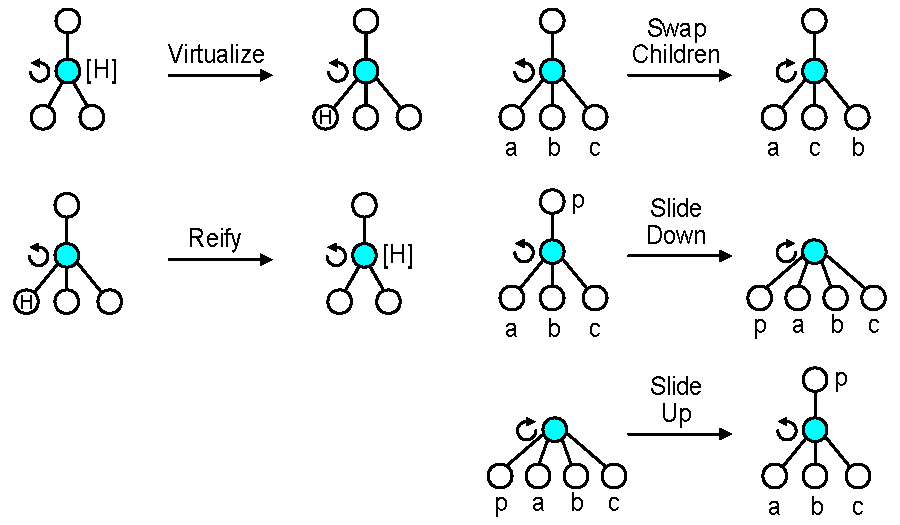
\includegraphics[width=\columnwidth]{configurational-transformations.pdf}
    \caption{Configurational Transformations.}
    \label{fig:configurational-transformations}
\end{figure}

Not all tetracoordinate atoms will be \textit{stereocenters}. A stereocenter is an atom whose \enquote{ligand permutation produces stereoisomers,} as defined by Mislow and Siegel~\cite{mislow:1984}. The presence of four bonds around a central atom is therefore a necessary, but insufficient condition. Molecular topology can result in permutation that does not yield stereoisomers. The assignment of non-default parities to such atoms should therefore be avoided.

Special handling is required for \textit{undefined stereocenters}. A stereocenter is undefined if it lacks a parity. Undefined stereocenters indicate that no information about a central atom's configuration is known. This could indicate the presence of either a single configuration or a configurational mixture. This interpretation is consistent with the one used by molfile format~\cite{ctfileFormats}.

\section*{Syntax}

A Balsa string is a sequence of zero or more characters belonging to the US-ASCII set (Figure~\ref{table:character-set}). The internal structure of a string reflects a depth-first traversal of the corresponding molecular graphs. As such, the syntax supports branches, cycles, and disconnected components.

\begin{table}
\caption{Balsa's Character Set.}
\centering
\begin{tabular}{c c c c c c}
    \hline
    Code & Character & Code & Character & Code & Character      \\
    \hline
    35   & \ttt{\#}  & 67   & \ttt{C}   & 92   & \ttt{\char`\\} \\
    37   & \ttt{\%}  & 68   & \ttt{D}   & 93   & \ttt{]}        \\
    40   & \ttt{(}   & 69   & \ttt{E}   & 97   & \ttt{a}        \\
    41   & \ttt{)}   & 70   & \ttt{F}   & 98   & \ttt{b}        \\
    42   & \ttt{*}   & 71   & \ttt{G}   & 99   & \ttt{c}        \\
    43   & \ttt{+}   & 72   & \ttt{H}   & 100  & \ttt{d}        \\
    45   & \ttt{-}   & 73   & \ttt{I}   & 101  & \ttt{e}        \\
    46   & \ttt{.}   & 75   & \ttt{K}   & 102  & \ttt{f}        \\
    47   & \ttt{/}   & 76   & \ttt{L}   & 103  & \ttt{g}        \\
    48   & \ttt{0}   & 77   & \ttt{M}   & 104  & \ttt{h}        \\
    49   & \ttt{1}   & 78   & \ttt{N}   & 105  & \ttt{i}        \\
    50   & \ttt{2}   & 79   & \ttt{O}   & 107  & \ttt{k}        \\
    51   & \ttt{3}   & 80   & \ttt{P}   & 108  & \ttt{l}        \\
    52   & \ttt{4}   & 82   & \ttt{R}   & 109  & \ttt{m}        \\
    53   & \ttt{5}   & 83   & \ttt{S}   & 110   & \ttt{n}       \\
    54   & \ttt{6}   & 84   & \ttt{T}   & 111   & \ttt{o}       \\
    55   & \ttt{7}   & 85   & \ttt{U}   & 112   & \ttt{p}       \\
    56   & \ttt{8}   & 86   & \ttt{V}   & 114   & \ttt{r}       \\
    57   & \ttt{9}   & 87   & \ttt{W}   & 115   & \ttt{s}       \\
    61   & \ttt{=}   & 88   & \ttt{X}   & 116   & \ttt{t}       \\
    64   & \ttt{@}   & 89   & \ttt{Y}   & 117   & \ttt{u}       \\
    65   & \ttt{A}   & 90   & \ttt{Z}   & 121   & \ttt{y}       \\
    66   & \ttt{B}   & 91   & \ttt{[}   &       &               \\
    \hline
\end{tabular}
\label{table:character-set}
\end{table}

\subsection*{Grammar}

Strings conform to an \textit{LL(1) grammar} \cite{thain:2020}. An LL(1) grammar is a context-free grammar whose strings can be parsed one character at a time from left to right with at most one character of lookahead. Additionally, LL(1) grammars expand the leftmost non-terminal first. These features make LL(1) grammars such as the one used by Balsa a good fit for manually-written recursive descent parsers. LL(1) grammars can also be used as a basis for auto-generated parsers through packages such as ANTLR~\cite{parr:2014}. The full grammar for Balsa strings is available as a text file in this paper's Supporting Material.

Balsa's formal grammar is presented as a series of \textit{production rules} (aka \enquote{productions}). A production rule defines a transformation allowed under the grammar. These transformations collectively define the set of valid Balsa strings. Production rules can be used in the forward direction, when writing a string, or in the reverse direction, when reading a string. 

A production rule is composed of two kinds of elements: \textit{terminals} and \textit{non-terminals}. A terminal is a character literal (e.g., \enquote{A}). A non-terminal is a reference to another production rule. This reference occurs through a name, which appears to the left of a separator (\ttt{::=}) in a production rule. To the right of a separator appear the allowed terminals and non-terminals for the rule.

Consider a hypothetical language composed of variable-length sequences of the lowercase letter \enquote{a}. Such a language could be cast as the following two production rules:

\begin{lstlisting}
<text> ::= <a>*
<a>    ::= "a"
\end{lstlisting}

The quantifier (\ttt{*}) indicates that a text in this language consists of a sequence of zero or more instances of the production \ttt{<a>}. This production in turn is defined as a lowercase letter (\enquote{a}). Therefore, valid texts in this language include the empty string, \enquote{a}, \enquote{aa}, and \enquote{aaaaaa} to name a few.

\subsubsection*{Atom}

Atoms carry most of the information in a Balsa string. The non-terminal \ttt{<atom>} can be expressed using one of four variants.

\begin{lstlisting}
<atom> ::= <star> | <shortcut> | <selection> | <bracket>
\end{lstlisting}

The first variant, \ttt{<star>}, produces one terminal value, the asterisk character (\ttt{*}). This \enquote{star atom} represents an atom in which every attribute assumes its default value.

\begin{lstlisting}
<star> ::= "*"
\end{lstlisting}

The next atomic production rule, \ttt{<shortcut>} is a non-terminal selected from the list: \enquote{B}; \enquote{C}; \enquote{N}; \enquote{O}; \enquote{P}; \enquote{S}; \enquote{F}; \enquote{Cl}; \enquote{Br}; and \enquote{I.} An atom encoded in this way (\enquote{shortcut atom}) receives the corresponding symbol as the value for the \ttt{element} attribute. All other attributes retain their default values, except \ttt{hydrogens}, which is set to \ttt{Implicit}.

\begin{lstlisting}
<shortcut> ::= "B" "r"? | "C" "l"? | "N" | "O" | "P"
             | "S" | "F" | "I"
\end{lstlisting}

The third atomic production rule, \ttt{<selection>} is a non-terminal selected from the list: \enquote{c}; \enquote{n}; \enquote{o}; \enquote{p}; and \enquote{s.} An atom encoded in this way (\enquote{selected shortcut atom}) assigns the corresponding capitalized atom symbol to the \ttt{element} attribute, sets the \ttt{selected} attribute to \ttt{true}, and sets the \ttt{hydrogens} attribute to \ttt{Implicit}. All other atomic attributes retain their default values.

\begin{lstlisting}
<selection> ::= "b" | "c" | "n" | "o" | "p" | "s"
\end{lstlisting}

The fourth and most complex atomic production rule is \ttt{<bracket>} (\enquote{bracket atom}). Bracket can be used to set any atomic attribute. A bracket atom must be used for any atom whose \ttt{configuration}, or \ttt{charge} attributes assume non-default values, or whose \ttt{hydrogens} attributes equals anything other than \ttt{Implicit}. Attributes not set within the \ttt{<bracket>} production rule will leave the corresponding atomic values in their default states.

\begin{lstlisting}
<bracket> ::= "[" <isotope>? <symbol> <parity>?
              <virtual_hydrogen>? <charge>? "]"
\end{lstlisting}

The value of a bracket atom's \ttt{isotope} attribute is determined by the optional \ttt{<isotope>} non-terminal. It consists of between one and three digits encoding the integers 1-999. Leading zeros (e.g., \enquote{007}) are disallowed.

\begin{lstlisting}
<isotope> ::= <nonzero> <digit>? <digit>?
\end{lstlisting}

The values of a bracket atom's \ttt{element} and \ttt{selected} attributes are determined by the \ttt{<symbol>} production rule (\enquote{symbol}). Three non-terminal variants are supported. These three variants influence the \ttt{element} and \ttt{selected} attributes in different ways. The \ttt{<star>} variant leaves both attributes as their default values. The \ttt{<element>} variant assigns the \ttt{element} attribute to the corresponding value while leaving the \ttt{selected} attribute as its default value. The \ttt{<selection>} non-terminal sets the \ttt{element} attribute to the corresponding element and the \ttt{selected} attribute to \ttt{true}. For example, the selection sequence \enquote{p} would assign the atomic \ttt{element} and \ttt{selected} attribute to \ttt{P} and \ttt{true}, respectively.

\begin{lstlisting}
<symbol> ::= <star> | <element> | <selection>
\end{lstlisting}

Given the large number of variants within the \ttt{<element>} non-terminal, the following production rule only defines the first several. For a complete list of variants, see the full grammar in the Supporting Information.

\begin{lstlisting}
<element> ::= "A" ( "c" | "g" | "l" | "m" | "r" | "s"
            | "t" | "u" )
            | "B" ( "a" | "e" | "h" | "i" | "k" | "r" )?
            ...
\end{lstlisting}

The \ttt{parity} attribute of a bracket atom is determined by the \ttt{<parity>} non-terminal. Allowed values are \enquote{@} and \enquote{@@,} corresponding to the values \ttt{Counterclockwise} and \ttt{Clockwise}, respectively.

\begin{lstlisting}
<parity> ::= "@" "@"?
\end{lstlisting}

The \ttt{hydrogens} attribute of a bracket atom is controlled by the \\ \ttt{<virtual{\_}hydrogen>} non-terminal. It is comprised of the terminal \enquote{H} followed by an optional \ttt{<nonzero>} non-terminal. A digit appearing after the \enquote{H} terminal sets \ttt{hydrogens} to the corresponding virtual hydrogen count. If no digit is present, \ttt{hydrogens} is set to one. The virtual hydrogen count is set to zero by omitting the \ttt{<virtual{\_}hydrogen} non-terminal.

\begin{lstlisting}
<virtual_hydrogen> ::= "H" <nonzero>?
\end{lstlisting}

The \ttt{<charge>} production rule sets the \ttt{charge} attribute of a bracket atom. This non-terminal begins with either the plus or minus terminals (\enquote{+} and \enquote{-} respectively) and ends with an optional \ttt{<nonzero>} non-terminal. A missing digit causes the atomic \ttt{charge} attribute to be set to one. In other words, the plus terminal (\enquote{+}) sets the \ttt{charge} attribute to one and the minus terminal (\enquote{-}) sets it to minus one. Charge values of zero are obtained if \ttt{<charge>} production is omitted.

\begin{lstlisting}
<charge> ::= ( "+" | "-" ) <nonzero>?
\end{lstlisting}

Values not defined within a bracket production leave the atomic attributes of the atom built from it in as their default values. For example, the bracket sequence \enquote{[C@H+]} lacks the \ttt{<isotope>} non-terminal so the value of the \ttt{isotope} attribute will remain as \ttt{None}. Similarly, the bracket sequence \enquote{[13CH+]} lacks the \ttt{<parity>} non-terminal, so the corresponding \ttt{parity} attribute remains \ttt{None}.

\subsection*{Sequence}

Children are added to an atom through the \ttt{<sequence>} non-terminal (\enquote{sequence}). A sequence starts with a required \ttt{<atom>} non-terminal. If no allowed non-terminals follow, the corresponding atom will have no children. Allowed non-terminals are chosen from the list: \ttt{<union>}; \ttt{<branch>}; and \ttt{<split>}.

\begin{lstlisting}
<sequence> ::= <atom> ( <union> | <branch> | <split> )*
\end{lstlisting}

The \ttt{<union>} non-terminal consists of an optional \ttt{<bond>} non-terminal followed by a mandatory non-terminal selected from the list: \ttt{<gap>} or \ttt{<sequence>}. If either of these latter non-terminals are detected but \ttt{<bond>} is not, the resulting bond is elided.

\begin{lstlisting}
<union> ::= <bond>? ( <bridge> | <sequence> )
\end{lstlisting}

The \ttt{<bond>} non-terminal supports five variants (\enquote{-,} \enquote{=,} \enquote{\#,} \enquote{/,} and \enquote{\textbackslash}). The first three (\enquote{-,} \enquote{=,} and \enquote{\#}) set the \ttt{order} attribute of a bond to one, two, or three, respectively. The last two terminals, \enquote{/} and \enquote{\textbackslash,} set the \ttt{order} attribute to 1 while also setting the \ttt{direction} attribute to \ttt{Up} and \ttt{Down}, respectively.

\begin{lstlisting}
<bond> ::= "-" | "=" | "#" | "/" | "\"
\end{lstlisting}

A sequence can contain a union, which in turn can contain a sequence. This is an example of recursion, transitive though it may be. Although left-recursion is disallowed in LL(1) grammars, right recursion of the kind in \ttt{<sequence>} is allowed. Right recursion also occurs within the \ttt{<union>} and \ttt{<branch>} non-terminals.

The \ttt{<bridge>} non-terminal (\enquote{bridge}) can take two forms. A digit non-terminal can be used, enabling single-digit bridge indexes in the range one through nine, inclusive. Double-digit bridge indexes, supporting the values ten through 99 inclusive, are available by prepending the percent character (\ttt{\%}). For the latter variant, leading zeros are disallowed, meaning that the sequence \enquote{\%07} must generate an error.

\begin{lstlisting}
<bridge> ::= <nonzero> | "%" <nonzero> <digit>
\end{lstlisting}

As noted previously, the purpose of a bridge is to create a bond without creating a connection within the molecular tree (see: \nameref{molecular-tree}). A bridge will most commonly be used to encode a ring-closure bond, but can be used anywhere within a string. The only requirement is that a bridge must be paired with another bridge having the same index. To prevent overflow, a bridge index may be reused.

An alternative to \ttt{<union>} within a sequence is the \ttt{<branch>} non-terminal (\enquote{branch}). Like union, branch joins a parent and child node through a bond. Wrapped by opening and closing parenthesis terminals (\enquote{(} and \enquote{)} respectively), branch encodes a sequence that may or may not be bonded to its parent. Bonding occurs if the \ttt{<bond>} non-terminal is included. Alternatively, the sequence will not be bonded if the \ttt{<dot>} non-terminal (\enquote{.}) appears. If neither \ttt{<bond>} nor \ttt{<dot>} are present then bond to the first atom of the sequence is elided.

\begin{lstlisting}
<branch> ::= "(" ( <dot> | <bond> )? <sequence> ")"
\end{lstlisting}

The third option for adding atoms within a sequence is the \ttt{<gap>} non-terminal (\enquote{gap}). A gap is a sequence of \ttt{<dot>} and \ttt{<sequence>} productions. The \ttt{<gap>} non-terminal serves the same purpose as it does within a branch: to enable connection within a molecular tree without creating a bonding relationship.

\begin{lstlisting}
<gap> ::= <dot> <sequence>
\end{lstlisting}

Having defined sequence, it's now possible to define a string as an optional sequence. In other words, a Balsa string is either empty or contains a sequence. A string without a sequence encodes a molecular tree having zero nodes and zero edges.

\begin{lstlisting}
<string> ::= <sequence>?
\end{lstlisting}

\section*{Implementation}

\subsection*{Reading Strings}
\label{reading-strings}

The goal of a Balsa reader is to transform a string input into a data structure output consistent with the string's content. The output data structure can take many forms. For example, a reader can merely validate a string by returning a boolean type. A more sophisticated reader can return a molecular graph capturing all atom and bond attributes and connectivity relationships.

Balsa strings are read one character at a time starting at the leftmost character and finishing at the rightmost character. The first character sets an initial reader state, and each subsequent character causes a state transition. The cumulative application of these state transitions yields the data structure to be returned.

Readers that capture atom-atom connectivity will typically maintain a reference to a \textit{hub}. A hub is an atom to which the next node will be connected. On reading the first complete \ttt{<atom>} non-terminal, the corresponding atom is constructed and set as the hub. Subsequently processing a complete \ttt{<union>}, \ttt{<branch>}, or \ttt{<gap>} non-terminal triggers three changes: (1) a child node is constructed; (2) the child is connected to the current hub, unless a \ttt{<dot>} non-terminal intervenes; and (3) the hub is replaced with the child node if it is an atom.

The presence of a branch adds some nuances over a union. The leading open parenthesis terminal (\enquote{(}) signifies that the current hub will later be re-exposed. This operation can be supported by a \textit{stack} (Table~\ref{table:stack-for-branches}). A stack is a data structure that allows items to be added individually and removed (\enquote{popped}) in the reverse order of addition. At the start of a branch, the current hub is pushed to the stack. At the end of the branch, the stack is popped and its top value is assigned as the new hub.

\begin{table}
    \caption{Stack and hub for reading the string \enquote{C(N*)O}.}
    \centering
    \begin{tabular}{c c l c c}
        \hline
        Step & Character   & Action                          & Hub & Stack \\
        \hline
        1    & \enquote{C} & create atom                     & C   &       \\
        2    & \enquote{(} & push next atom                  & C   &       \\
        3    & \enquote{N} & create atom, push atom          & N   &  N    \\
        4    & \enquote{*} & create atom                     & *   &  N    \\
        5    & \enquote{)} & pop atom, update hub            & N   &       \\
        6    & \enquote{O} & create atom                     & O   &       \\
        \hline
    \end{tabular}
    \label{table:stack-for-branches}
\end{table}

Additional modifications allow bridge bonds to be tested for \textit{compatibility} (Figure~\ref{fig:bridge-bond-compatibility}). Compatibility is tested by comparing the attributes of each bridge bond. This test has three parts:

\begin{enumerate}
    \item An elided bond is compatible with any other bond.
    \item A bond with a non-default direction is only compatible with an elided bond or a bond of opposite direction.
    \item A bond with default direction is only compatible with an elided bond or a bond of identical order and default direction.
\end{enumerate}

A workflow modification allows bridge bonds to be compared for compatibility. A 100-element array is used to maintain state. The first occurrence of a bridge causes the bridge bond's attributes to be copied to the array at the bridge index. The second occurrence of a bridge causes the entry to be removed. The attributes stored in the entry are then compared with those of the current bridge bond. If the two sets of attributes are incompatible, an error must be reported.

\begin{figure}
    \centering
    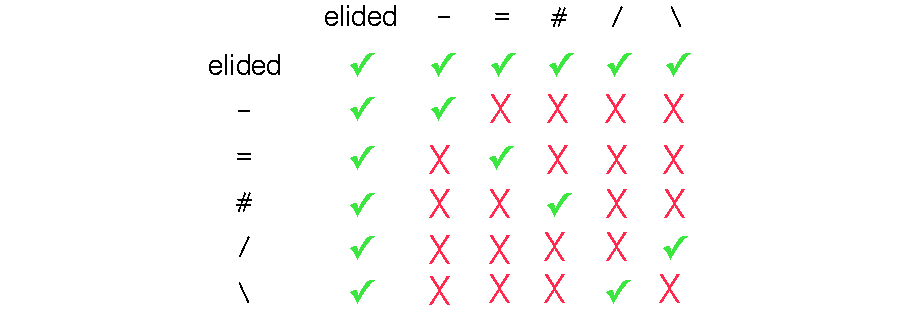
\includegraphics[width=\columnwidth]{brdige-bond-compatibility.pdf}
    \caption{Bridge bond compatibility. Two bonds with the types indicated along the row and column headings are either compatible (green check marks) or incompatible (red X).}
    \label{fig:bridge-bond-compatibility}
\end{figure}

An elided bond is compatible with any other bond (Rule 1). Unless both bridge bonds are elided, however, the presence of compatible but unmatched bridge bonds could interfere with atom-centered computations. One solution is to set the attributes of the elided bridge bond explicitly. The array used for compatibility testing can be re-used to set the attributes of an unmatched bridge bond pair.

Readers must not assume that a dot (the period terminal, \enquote{.}) implies the presence of disconnected components. This assumption is most likely to arise in the context of ad-hoc parsers using regular expressions, string matching, and the like. For example, the connected molecular graph for propane can be encoded using the string \enquote{C1C.C1}.

A reader must assume that any input string can contain errors, and take appropriate steps to report them. The most useful errors will report a specific cause. Some will also report one or more cursor indexes. The most common mandatory errors are:

\begin{enumerate}
    \item{Invalid character (position). An unexpected character was encountered. A list of acceptable characters is helpful, but not required.}
    \item{Unexpected end-of-line. Input ended unexpectedly.}
    \item{Unbalanced bridge (position). A bridge with a given index appears an odd number of times.}
    \item{Incompatible bridge bonds (position, position). The bonds to a pair of cuts are incompatible.}
    \item{Delocalization subgraph lacks perfect matching. Before reporting this error, steps to remove unnecessarily selected atoms should be taken as described in the next section.}
    \item{Partial parity bond not allowed (position). Neither terminal of a PPB possesses a double bond. Strings such as \enquote{C/C} and \enquote{C{\textbackslash}C} contain isolated PPBs, which are invalid. A reader encountering such strings must report an error.}
\end{enumerate}

A reader may also report optional errors, including:

\begin{enumerate}
    \item{Impossible isotope. A negative implied mass number results from the atom (e.g., \enquote{[2C]}).}
    \item{Impossible valence. The valence at an atom is impossibly high (e.g., \enquote{C(C)(C)(C)(C)C}).}
    \item{Impossible charge. An atom's charge gives it an apparent negative electron count (e.g., \enquote{[C+7]}).}
\end{enumerate}

\subsection*{Pruning}

As noted previously, a delocalization subgraph is invalid if it lacks a perfect matching. The one exception is when a selected atom and its associated bonds can be deleted from the delocalization subgraph through \textit{pruning}. Pruning unsets the \ttt{selected} attribute of a selected atom without corresponding promotion of any attached bonds.

An atom must be pruned if its subvalence equals zero. None of the bonds to such an atom can be promoted without altering the atom's \ttt{charge} attribute. Pruning the atom ensures the stability of its \ttt{charge} attribute, without interfering with bond promotion elsewhere. Viewed from another perspective, an atom with zero subvalence lacks unpaired electrons - at least within the narrow boundaries of the Balsa valence model. Such atoms can only form double bonds through changes to atomic charge. 

If a selected atom bears a non-zero \ttt{charge} attribute, subvalence is computed using the isoelectronic element's default valences. For example, a selected nitrogen atom with a charge of +1 would use the default valences for carbon. A selected phosphorous atom with a charge of -1 would use the default valences of sulfur. And so on. If no default valences are found in this way (e.g., \enquote{[c+2]}), a reader must report an error. Writers must not encode such atoms.

\begin{figure}
    \centering
    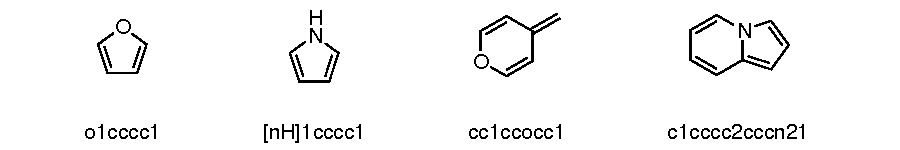
\includegraphics[width=\columnwidth]{gratuitous-selection.pdf}
    \caption{Gratuitous selection. Heteroatoms are selected needlessly because subvalence is zero in every case. Atoms selected gratuitously, must be pruned before processing the DS.}
    \label{fig:gratuitous-selection}
\end{figure}

Pruning becomes necessary in cases of \textit{gratuitous selection} (Figure~\ref{fig:gratuitous-selection}). Gratuitous selection is the selection of an atom whose subvalence is zero and which therefore can never become part of a DS. This can happen when style, tradition, or convenience override symmetry concerns. Consider a string representing furan in which all atoms are selected (e.g., \enquote{c1ccco1}). Selecting any atom is unnecessary because furan does not exhibit DIME. This applies doubly to the the oxygen atom because it lacks an unpaired electron and so will never lead to DIME. It is nevertheless convenient to select the carbon atoms because all bonds can then be elided. The resulting representation (e.g., \enquote{c1cccO1}) leads to a delocalization subgraph with a perfect matching and hydrogen counts consistent with the original encoding.

Writers are encouraged, but not required, to avoid gratuitous atom selection. Readers, however, must always be prepared to prune.

\subsection*{Writing Strings}

Whereas a reader transforms a string into a data structure, the goal of a writer is the opposite: to transform a data structure into a valid string. This data structure will most commonly take the form of a molecular graph or tree, but other forms are possible. For practical reasons, the input data structure is likely to resemble the output from a reader. Such an arrangement makes it possible to encode and decode strings with minimal intermediate translation.

Regardless of the form taken by the input data structure, it must be traversable in \textit{depth-first} order (Figure~\ref{fig:depth-first-traversal}). A depth-first traversal operates over a set of nodes bound by a set of connectivity relationships, which are typically edges. Traversal proceeds by successively replacing each node as the center of focus, or root. Each new root is chosen from the untraversed neighbors of the current root. Eventually all nodes are processed, ending the traversal.

\begin{figure}
    \centering
    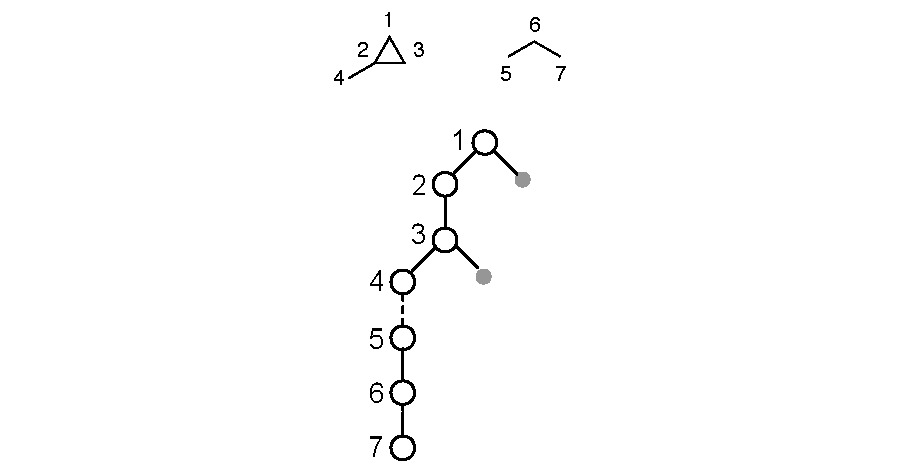
\includegraphics[width=\columnwidth]{depth-first-traversal.pdf}
    \caption{Depth-first traversal. Traversal of a disconnected, cyclic molecular graph (top) in depth-first order leads to a tree containing one bridge and one gap (bottom).}
    \label{fig:depth-first-traversal}
\end{figure}

A writer intercepts the depth-first traversal of an input data structure to write an output string compatible with the formal grammar. There are no requirements around style. For example, it's equally valid to represent the carbon atom of methane using either implicit or virtual hydrogens (e.g., \enquote{C} or \enquote{[CH4]}). Single bonds may be elided or not, all other things being equal. Similarly, the DS may or may not be empty. Although an organization may seek to standardize certain styles of string output, any syntactically and semantically valid string must be considered valid by a reader.

The presence of branches within an input data structure is encoded via the \ttt{<branch>} non-terminal. A useful tool for this purpose is a stack (Table~\ref{table:stack-for-writing-string}). A writer begins by pushing the current branch onto the stack and extending it. When a new branch is encountered, it is pushed to the stack and extended. When the branch terminates, the current branch is popped and its contents are appended to the stack's new top item.

\begin{table}
    \caption{Writing a string with the aid of a stack.}
    \centering
    \begin{tabular}{c}
        
\includegraphics[width=\columnwidth]{tree-for-stack.pdf}
    \end{tabular}

    \bigskip

    \begin{tabular}{c l l}
        \hline
        Step & Action & Stack \\
        \hline
        1  & root C   & \enquote{C}                             \\
        2  & open     & \enquote{C},\enquote{(}                 \\
        3  & extend N & \enquote{C},\enquote{(N}                \\
        4  & open     & \enquote{C},\enquote{(N},\enquote{(}    \\
        5  & extend S & \enquote{C},\enquote{(N},\enquote{(S}   \\
        6  & extend I & \enquote{C},\enquote{(N},\enquote{(SI}  \\
        7  & close    & \enquote{C},\enquote{(N(SI)}            \\
        8  & extend F & \enquote{C},\enquote{(N(SI)F}           \\
        9  & close    & \enquote{C(NSI)F)}                      \\
        10 & extend O & \enquote{C(NSI)F)O}                     \\
        \hline
    \end{tabular}
    \label{table:stack-for-writing-string}
\end{table}

Writers should consider the non-negligible costs of atom selection. Algorithms for selection are likely to involve the perceptions of cycles, and could exhibit superlinear time complexity. Often, a reader must perform a global deselection to arrive at a localized valence bond representation, which at the very least requires pruning and a maximal matching procedure. In other words, atom selection imposes two sets of costs: one on the writer and the other on every subsequent reader forever into the future.

Writers must ensure that all selected atoms can be deselected. Consider pyrrole, erroneously encoded with a selected nitrogen atom (e.g., \enquote{n1cccc1}). The nitrogen atom can not be pruned because of its non-zero subvalence (3 - 2). The DS therefore contains all five atoms and all five bonds. A perfect matching does not exist. A reader receiving such a string must report an error. To avoid this outcome, a writer can consume the subvalence by adding a virtual hydrogen (e.g., \enquote{[nH]1cccc1}). The subvalence of nitrogen in this case is zero, so the atom can be pruned. Doing so leaves a DS with four atoms, four edges, and a perfect matching. Readers will therefore consider the string valid. The larger question of gratuitous selection nevertheless remains.

\subsection*{Working with Molecular Graphs}
\label{working-with-molecular-graphs}

Molecular trees offer some important advantages, but they are used less often than molecular graphs. Sooner or later, it will be necessary to interconvert the two representations when using Balsa. Readers will need to transform a tree into a graph, and writers will need to transform a graph into a tree. Although there are only three main differences between molecular trees and molecular graphs, these differences can lead to subtle effects during transformation. Understanding these effects is the key to lossless conversion.

The first difference is the simplest to account for: atoms in a molecular tree have two kinds of edges: the one entering from an optional parent; and the zero or more exiting to children. A molecular graph, in contrast, maintains a single set of edges for an atom. Transformation of an atom in a tree to one in a graph must account for a possible inbound bond. The converse transformation must place the inbound bond.

The second difference is that molecular trees have gaps, but molecular graphs do not. An edge may or may not represent a bonding relationship. Transformation from tree to graph must recognize the presence of gaps and place no corresponding bond. Gaps can occur at any outbound edge, even those within branches. Transformation from graph to tree must locate an appropriate pair of atoms to host the gap. A convenient pair would be the last atom of the first connected component and the first atom of the next connected component, but other choices are possible.

The third difference leads to the most complex reconciliation: molecular trees have bridges but molecular graphs do not. When transforming tree to graph, the two sides of a bridge bond must be identified, spliced, and added to the graph. When transforming graph to tree, a ring closure bond must be detected and split into a pair compatible bridge bonds. Compounding the problem in either sense of conversion is index reuse. Transformation from graph to tree will reuse gap indexes to avoid overflow. Transformation from tree to graph must account for the possibility that gap index reuse has occurred.

Transformation of graph to tree can be aided by a \textit{pool} (Tabe~\ref{table:pool}). A pool issues a bridge index given an unordered pairing of atomic identifiers. The bridge index will not be re-issued until the pool receives the same pairing again. A pool is used during a depth-first traversal of a molecular graph, where the presence of a cycle is indicated by the discovery of an index that has already been traversed. On encountering a cycle, a bridge index is requested from the pool by submitting the source and target atomic indexes as an unordered pair. The bridge index is then used to construct the first half of the gap bond. Later, the same bond will be traversed in the opposite direction. When it is, a gap index is requested from the pool by re-submitting a source and target index pairing. Doing so yields the bridge index, while simultaneously freeing it for later use.

\begin{table}
    \caption{A pool manages bridge indexes during the transformation of a molecular graph.}
    \centering
    \begin{tabular}{c}
        
\includegraphics[width=\columnwidth]{pool.pdf}
    \end{tabular}

    \bigskip

    \begin{tabular}{c l l l l}
        \hline
        Step & Edge  & Hit & Return Value & Action    \\
        \hline
        1    & (0,1) & No  & None         &           \\
        2    & (1,2) & No  & None         &           \\
        3    & (2,3) & No  & None         &           \\
        4    & (3,0) & Yes & 1            & Reserve 1 \\
        5    & (3,1) & Yes & 2            & Reserve 2 \\
        6    & (1,3) & Yes & 2            & Release 1 \\
        7    & (1,4) & No  & None         &           \\
        8    & (4,5) & No  & None         &           \\
        9    & (5,6) & No  & None         &           \\
        10   & (6,4) & Yes & 2            & Reserve 2 \\
        11   & (4,6) & Yes & 2            & Release 2 \\
        12   & (0,3) & Yes & 1            & Release 1 \\
        \hline
    \end{tabular}
    \label{table:pool}
\end{table}

\section*{Compatibility}

For maximum compatibility with existing software, Balsa was designed as a \textit{language subset} of SMILES. A language subset contains some of the syntax and semantics of its parent language, but adds none of its own. In principle this means that a feature present in Balsa should also be present in SMILES. Conversely, a feature present in SMILES may or may not also be present in Balsa.

Language subsets have ample precedent in computer science. A well-known example is MISRA C~\cite{misraC}, a subset of the C programming language that aims to eliminate \enquote{known undefined or otherwise dangerous behavior}~\cite{hatton:2007}. Another example is the subset of JavaScript described by Crockford whose purpose is to \enquote{chip away at the features that are not beautiful until the language's true nature reveals itself.}~\cite{crockford:2008}. Language subsets arise for two main reasons. First, designing a language presents many opportunities to introduce errors small and large. Second, popular languages inevitably bring with them many users with diverse problems that demand new features. Some of these features cause future problems of their own. A language subset can improve both situations by eliminating the most problematic features.

Although similar considerations apply to SMILES, its case is different in one important way: SMILES was never publicly described with high precision. Overviews of the language have been published by both Weininger and Daylight. But the kind of technical documentation suitable for software development was never made public. Both the OpenSMILES and SMILES+ initiatives cite this shortfall as motivation.

Nevertheless, several SMILES software implementations have been released as noted previously. Each one represents its own unique set of decisions about how to reduce the published broad SMILES descriptions to a specification detailed enough for software development. Some implementations have themselves been reverse-engineered for clues. The Daylight implementation in particular is sometimes invoked as a de facto SMILES specification. Unfortunately, access to this implementation is restricted by commercial licensing, as is the case with several SMILES implementations. Moreover, reverse engineering is unlikely to address every question because of the vast search space embodied by SMILES. Although some implementations are released under Open Source licenses, they are neither authoritative nor unanimous in their interpretations.

A publicly-available and precise subset of SMILES would offer a new way to address the problem. If sufficiently constrained, the subset should be interpretable by all existing software without modification. Moreover, most strings written by existing software would be interpretable by software based on the language subset. Because its description would be both public and precise, the language subset could serve as the basis for many implementations with strong consensus around both syntax and semantics.

Unfortunately, the choice of the Balsa base language is fraught with difficulty on technical, historical, and cultural grounds. Simply put, the term \enquote{SMILES} has come to mean different things to different people. To some, SMILES is the language defined in public documentation. To others, SMILES is the Daylight implementation source code. Some may view SMILES as the collective definitions contained in both published documents and all software. To others, SMILES isn't even definable.

These problems can be avoided by considering as a base language not SMILES itself, but a \textit{proto-language}. A proto-language is a hypothetical language from which a family of languages can be derived. A suitable SMILES proto-language would ideally contain all of the features consistent with the many ways in which the term \enquote{SMILES} is used today.

Accordingly, Balsa's base language is \enquote{ProtoSMILES,} a SMILES proto-language. ProtoSMILES was identified through a process of elimination that started with every SMILES document ever published and every SMILES software implementation. The field was narrowed through two limitations: (1) the source must be authoritative; and (2) the source must be publicly accessible. "Authoritative" means that the source was created by either Weininger himself or Daylight, who alone can speak most authoritatively about what SMILES is. The requirement for public accessibility ensures that claims of compatibility can be tested. The following documents were identified as candidate ProtoSMILES sources:

\begin{itemize}
    \item Weininger's report to the US Environmental Protection Agency (\enquote{The Report})~\cite{anderson:1987}.
    \item Weininger's original publication (herein \enquote{The Article})~\cite{weininger:1988}.
    \item Weininger's 2003 book chapter, revised in 2008 (\enquote{The Chapter})~\cite{weininger:2003}.
    \item An online manual maintained by Daylight (\enquote{The Manual}).
    \item The Daylight's toolkit, which implements a SMILES reader and writer (\enquote{The Toolkit})~\cite{daylightToolkit}.
\end{itemize}

The Toolkit was eliminated for three reasons. First, its source code is not available, forcing an indirect reverse-engineering approach to language definition. Second, as a product of the company Weininger started, the Toolkit is likely to recapitulate the other sources. Third, as a commercial product without source code, the Toolkit may not always be available in the future.

The Report was eliminated mainly because the contents of this older document contradict at least two of the remaining sources (The Article and the Chapter). The Report contains no mention of bracket syntax, using markedly different notation instead. The Report also supports unusual characters including the exclamation mark (\ttt{!}). Unspecified \enquote{special states} for nitrogen-containing atoms are also supported by the Report.

The Manual was disregarded as a ProtoSMILES source because it merely restates content already present in The Paper and The Chapter. Removing this source simplifies the construction of ProtoSMILES without changing its definition. A secondary consideration was the possibility that updates to this web page could change the meaning of ProtoSMILES. However, web archives indicate that neither styling nor content of the Manual have changed in at least ten years.

Careful reading of The Article and The Chapter reveals the former to contain all of the material in the latter. Moreover, The Chapter contains information not present in The Article. Therefore, the Paper was eliminated as a basis for ProtoSMILES.

This process of elimination leaves just The Chapter as the basis for ProtoSMILES. The remainder of this section compares and contrasts ProtoSMILES with Balsa. The main difficulty with this approach is that the work defining ProtoSMILES occasionally contains contradictions. These will be noted when relevant.

ProtoSMILES defines a fixed set of element symbols that even at the time of publication was partially obsolete~\cite[p.~83]{weininger:2003}. The symbol for element 105 is given as Ha (Hahnium), despite IUPAC's resolution of the naming controversy of the element in favor of the symbol Db (Dubnium) years prior~\cite{sageson:1997}. Balsa therefore disallows the symbol Ha. To maintain compatibility with ProtoSMILES and avoid future changes to Balsa's grammar, elements after element 105 are also excluded.

ProtoSMILES defines a recursive grammar for branching which, perhaps without the knowledge of the author, allows sequentially nested parentheses~\cite[p.~86]{weininger:2003}. Balsa disallows such constructs (e.g., \enquote{*((*))*} and \enquote{*(((*)))*}).

ProtoSMILES supports reactions but Balsa does not. Specifically, the greater than symbol (\ttt{$>$}) is not a valid Balsa character. This restriction precludes strings such as \enquote{*$>$$>$*}. Furthermore, Balsa lacks the \enquote{map} attribute, used for atom-atom mapping in reactions, and its accompanying syntax.

Balsa only supports two stereodescriptors, encoded with the terminals \enquote{@} and \enquote{@@.} ProtoSMILES provides a recursive grammar for stereodescriptors that allows multi-symbol descriptors such as \enquote{@@@} and \enquote{@@@@}~\cite[p.~94]{weininger:2003}. ProtoSMILES also supports non-tetrahedral descriptors including \enquote{@AL1,} \enquote{@AL2,} \enquote{@1,} and \enquote{@SP1.} None of these are supported by Balsa. Nor does Balsa support the application of tetracoordinate stereodescriptors to odd cumulenes. These other forms of atomic configuration are relatively rare. Their inclusion in Balsa would add substantial cost for minor payoff.

ProtoSMILES supports \enquote{aromatic bonds} (\enquote{:}), but Balsa does not. Despite clear inclusion within the syntax of ProtoSMILES, no precise guidance on using aromatic bonds is provided. Weininger notes that \enquote{Adjacent atoms without an intervening bond symbol are connected by a valence-dictated bond (typically a single or aromatic bond) \enquote{-} (single) and \enquote{:} (aromatic) bond symbols may always be omitted on input}~\cite[p.~85]{weininger:2003}. This passage implies that aromatic bonds serve no purpose. Accordingly, Balsa does not allow them and the syntax does not include the colon symbol (\ttt{:}).

% ProtoSMILES appears to allow ANY element to be made lower case!

ProtoSMILES sets no limits on the atoms that can be marked as selectable (i.e., \enquote{aromatic}), but Balsa does. As described previously, pruning the DS requires a method to determine whether or nor an atom is subvalent (see: \nameref{valence-and-subvalence}). Making this determination requires at least one default valence. The only reasonable way to allow selection of all atoms regardless of associated element would be to provide default valences. As a result, only those atoms associated with a subset of elements may be selected (\enquote{B}, \enquote{C}, \enquote{N}, \enquote{O}, \enquote{P}, \enquote{S}). This list is a subset of the elements whose default valences are defined. Halogens were excluded because they rarely appear in rings. This restriction only marginally limits the capabilities of Balsa because atoms other than those supported are rarely involved in DIME.

It's unclear whether ProtoSMILES allows a virtual hydrogen count on hydrogen itself. Weininger notes that \enquote{explicit hydrogen specification is required} in the case of \enquote{hydrogens connected to other hydrogens, e.g. [H][H], molecular hydrogen}~\cite[p.~97]{weininger:2003}. This may reflect an erroneous belief that parsers would be incapable of processing strings such as \enquote{[HH]}. To be clear, Balsa supports virtual hydrogen counts on all atoms.

ProtoSMILES ascribes ambiguous meaning to gaps. As noted by Weininger, \enquote{... In terms of the valence model being represented, the dot literally represents a bond of formal order zero: the atoms on either side of the dot are explicitly not bonded to each other.}~\cite[p.~88]{weininger:2003}. Other statements appear to contradict this statement. Balsa explicitly disallows the zero bond order interpretation.

ProtoSMILES assigns no explicit upper or lower bounds to numerical atomic attributes. These boundaries are nevertheless crucial for implementors, who must determine the data types necessary to efficiently prevent underflow and overflow. For this reason, Balsa sets both upper and lower bounds, respectively, on the following atomic attributes: isotope (0 $<$ value \textless 1000); charge (-10, \textless value \textless 10); and hydrogens, 0 $\leq$ value \textless 10). Although it might be argued that lower bounds on physical quantities such as isotope and hydrogen count should be implicit, the lack of precision forces implementors to improvise, which can lead to divergent behavior. ProtoSMILES places no upper bound on the charge notation (e.g., \enquote{++} and \enquote{-{}-}): \enquote{\dots \enquote{+} meaning +2 \dots}~\cite[p.~94]{weininger:2003}. Due to their redundancy, Balsa disallows duplicated plus and minus characters (\ttt{+} and \ttt{-}, respectively) within bracket atoms.

Balsa provides a few semantic clarifications not fully addressed in ProtoSMILES. A detailed algorithm for determining implicit hydrogen count is provided, together with the required valence table. Unlike ProtoSMILES, Balsa explicitly considers the case of computing implicit hydrogen counts on selected atoms. Balsa also provides detailed algorithms, absent in SMILES, for selection and deselection. These are based in graph theory rather than the ambiguous and overloaded chemical concept of \enquote{aromaticity} used in ProtoSMILES. Uniquely, Balsa introduces the concepts of \enquote{pruning} and \enquote{gratuitous selection.} ProtoSMILES does not specify those bonds that can be promoted during deselection, but Balsa does. ProtoSMILES does not restrict partial parity bonds to those atoms also possessing at least one double bond, whereas Balsa does. Finally, Balsa syntax is based on a formal grammar and tooling rooted in decades of computer science research, whereas ProtoSMILES syntax is based for the most part on imprecise natural language descriptions and only a partial formal grammar.

\begin{table}
\begin{minipage}{\textwidth}
\renewcommand*\footnoterule{}
    \caption{Some differences between ProtoSMILES and Balsa.}
    \centering
    \begin{tabular}{p{0.50\linewidth} p{0.20\linewidth} p{0.15\linewidth}}
        \hline
        Feature & ProtoSMILES\footnote{Values of \enquote{maybe} indicate ambiguous and/or contradictory statements by Weininger.} & Balsa \\
        \hline
        element symbol Ha & yes & no \\
        multiple branching (e.g., \enquote{*((*))*}) & yes & no \\
        reactions using greater than symbol (\ttt{>}) & yes & no \\
        atomic \enquote{map} attribute & yes & no \\
        extended stereodescriptors (e.g., \enquote{@OH1}) & yes & no \\
        use of stereodescriptors on odd cumulene centers & yes & no \\
        virtual hydrogen count on hydrogen (e.g., \enquote{[HH]}) & maybe & yes \\
        detachments are bonds of \enquote{formal order zero} & maybe & no \\
        unbounded numerical atomic properties & yes & no \\
        atoms associated with any element are selectable & yes & no \\
        non-elided bonds may be promoted during selection & maybe & no \\
        isolated partial parity bond & yes & no \\
        repeated charge notation (e.g., \enquote{++} and \enquote{-{}-}) & yes & no \\
        aromatic bond (\enquote{:}) & yes & no \\
        \hline
    \end{tabular}
    \label{table:feature-comparison}
\end{minipage}
\end{table}

Compatibility between Balsa and ProtoSMILES is summarized in Table~\ref{table:feature-comparison}. Barring elements of ProtoSMILES that are either underspecified or internally inconsistent (entries marked \enquote{maybe}), Balsa can be seen to be a subset of ProtoSMILES. Output from Balsa writers should therefore be readable by SMILES readers. However, output from SMILES writers may or may not be readable by Balsa readers.

\section*{Discussion}

Balsa's main advantage as a molecular serialization format is high information density. The most common atom types can be represented with just one character. The worst case atom, using every available atomic attribute, requires 14 characters. The most common bond types can be encoded implicitly. In the worst case one character per bond is required.

These metrics compare favorably with alternatives. Consider the molfile (V2000) format. 32 characters per atom are required in the best case, and 51 characters in the worst. All bonds, regardless of type, require between nine and 12 characters. Atomic charges and isotopes typically require additional characters.

The information density of Balsa strings makes them attractive for several applications. In memory-constrained environments such as those found on handheld devices and network serialization, many more Balsa strings can be present than alternative encodings. In-memory structure search over large collections becomes feasible. Because a Balsa string often fits within one line on a terminal, it can be used for data entry in manual interactive shells such as a real-eval-print loops (REPLs) or notebooks.

Another advantage is lossless serialization and deserialization. The line notation InChI might appear to compete with Balsa in this sense. The authors of InChI have noted that InChI is not a solution to the molecular serialization problem but rather an identifier.\cite{heller:2015} The reason presumably lies with the fact that both serialization and deserialization require intimate knowledge of the InChI canonicalization algorithm. To date, no third-party reader or writer of InChI has ever been released.

Despite its information density, Balsa can faithfully encode and decode most of what chemists would consider \enquote{organic molecules.} This is evidenced by the widespread presence of Balsa strings within large, public-facing databases such as PubChem,\cite{kim:2016} ChEMBL,\cite{gaulton:2012} ChEBI,\cite{degtyarenko:2007} and others.

Balsa's compact representation requires some tradeoffs regarding expressiveness. Extended bonding beyond the delocalization subgraph is not supported. This limitation excludes many types of molecule, including organometallics and delocalization-\-stabilized ions. Zero-\-order bonds are not supported, making it difficult to accurately encode coordination complexes. Only four-\-coordinate, tetrahedral stereocenters can be encoded, excluding many forms of chirality, including helical chirality, all forms of non-\-tetrahedral stereochemistry, and lone-\-pair tetrahedral centers. Conformational restrictions beyond the isolated double bond are not supported, which excludes important molecules such as those exhibiting atropisomerism. Other formats such as CDXML and molfile support enhanced stereochemical features enabling the differentiation of various kinds of partial stereochemical information, but Balsa does not.

Broader expansion of Balsa's capabilities could be possible through \textit{metaformats}. A metaformat embeds one or more Balsa strings within a surrounding serialization format. For example, two- or three-dimensional coordinates could be associated with each atom through a metaformat that includes a dictionary mapping atomic index to coordinate. Collections of atoms or bonds could likewise be encoded to replicate the enhanced stereochemistry features of other formats. And so on. However, the utility of such extensions should be weighed against Balsa's main value proposition: high information density. An application attempting to use a verbose metaformat may benefit from adopting better-suited format instead.

Setting aside the many technical and usability issues a metaformat would raise, versioning is likely to play an important role. Balsa itself lacks any mechanism to convey the concept of version. This stands in contrast to InChI, which not only encodes a version identifier, but has done so from its first release. Adding a version identifier would, unfortunately, break compatibility with the large number of existing SMILES software. Metaformats offer an opportunity to address this limitation.

The most noteworthy feature of Balsa is its compatibility with SMILES. Contemporary SMILES implementations will be able to read and write Balsa strings --- at least to a point. Incompatibilities will arise from two main sources: (1) those features of SMILES that Balsa has deliberately omitted; and (2) those aspects of the SMILES language that are incompletely-specified, ambiguous, or self-contradictory.

The availability of a minimal yet highly functional, fully-specified core language offers many opportunities to improve data quality. One of the most important will be an open reference implementation, the design and source code of which will be discussed later. A freely-available reference implementation in turn makes automated validation suites possible. These suites can improve data quality by reporting syntax and semantic differences among implementations, preferably before release. A reference implementation taken together with the guidelines for readers and writers in this paper should make it possible to write software that conforms to a very high level of precision, regardless of programming language or paradigm. Given verified implementations, performance optimizations can be considered. The existence of a core language specification should also aid standardization efforts, either for Balsa itself, or SMILES. Finally, the development of better line notations is only possible given a thorough understanding of the scope and limitations of existing options. Here, metaformats could offer a bridge from the present to the future.

\section*{Conclusion}

This paper describes Balsa, a subset of the widely-\-used SMILES line notation. Balsa's features are detailed at four levels: constitution; delocalization; conformation; and configuration. Constitutionally, Balsa can encode any molecule conforming to the valence bond model. In the event of undesired symmetry artifacts due to delocalization, Balsa offers a mitigation based in graph theory. Conformational isomerism of alkenes is supported by partial parity bonds. The configurations of tetracoordinate, stereogenic atoms are encoded through the use of a parity enumeration and conventions around its use.

Balsa's syntax is described in detail through a formal grammar. This method concisely summarizes the complete set of strings that could be considered syntactically valid Balsa representations. The formal grammar was deliberately structured to be used either directly with an automated parser generator or with a hand-written recursive-descent parser.

The complete set of operations needed to interpret Balsa's syntax semantically are described in detail. This is a crucial component of the language's definition because Balsa achieves its information density largely by favoring convention over encoding. As an aid to difficult cases, guidelines for readers and writers are included.

As a subset of SMILES, Balsa can be used with a wide range of SMILES software today. In this sense, Balsa may seem to offer nothing new or even of value. However, Balsa has been defined at a level of detail that SMILES never was. This difference makes it possible to use Balsa in unique ways. Open reference implementations and validation suites can now be developed and deployed. Families of extensions can be built, each one based on the same unambiguous foundation. Formal standardization becomes more feasible given detailed reference material on which to draw. Finally, it is only through the clear demarcation of boundaries that the frontier becomes visible.

\clearpage
\printbibliography

\end{document}